\documentclass{article}
\usepackage{amssymb}
\usepackage{graphicx}
\usepackage{caption}
\usepackage{subcaption}
\usepackage{listings}
\usepackage{float} %figure inside minipage
\graphicspath{ {./images/} }
\usepackage[export]{adjustbox}
\usepackage{apacite}




\begin{document}
\begin{titlepage}
\author{Humaid Agowun and Paul Muir} 
\title{Performance Analysis of a Collection of ODE Solvers on Covid-19 Models with Discontinuities 
} 
\date{\today} 
\maketitle
\end{titlepage}

\begin{center}
    \textbf{Abstract}
\end{center}

In this report, we consider the numerical solution of two challenging
Covid-19 ordinary differential equation (ODE) 
models that have discontinuities. One of the models has a 
time-dependent, i.e., at a given point in time, a discontinuity is introduced
into the model. The second type of discontinuity is a state-dependent discontinuity;
this means that the time at which the discontinuity arises depends on the
value of one of the solution components, and thus it is not known apriori.

These discontinuities make the models quite challenging for standard ODE solvers.
Furthermore, the presence of exponentially growing solution components adds further
to the difficulties faced by standard ODE solvers when trying to solve these types of 
problems.

We report on an investigation of performance of a wide array of ODE solvers (we
consider 21 solvers) available in four major software environments: R, Python, 
Scilab, and Matlab, applied to these models.

We focus on straightforward implementations of the models within the above environments
where the user employs the solvers and codes the problems using default settings for 
the solvers, e.g., default tolerances, and simple implementations for the
discontinuities, e.g., the introduction of if-then statements into the functions that 
define the right-hand sides of the ODE systems. Such implementations of the models
and usage of the solvers are typical of what researchers might employ.

We also include an investigation of the solution of the models using slightly more
sophisticated, but easily implementable, treatments of the models; these treatments
involve making better use of the capabilities of the solvers, and slightly more careful
implementations of the models themselves.

We also highlight a number of issues with the way that some of the solvers are implemented
in some of the software environments. For example, the way in which output points, where 
the user specifies points in the domain where the solution value should be provided,
is an issue in some of the software environments. 

{\it We show that the standard use of ODE solvers available within  widely used software 
environments, applied to simple implementations of these Covid-19 models, will
frequently deliver numerical solutions that have no significant digits of accuracy.
Furthermore, the solvers give no indication that the return solutions
may be inaccurate.} We also show that the straightforward treatments of the models 
are always less efficient than the slightly more sophisticated treatments.
{\it We show that the slightly more sophisticated treatments of the models can 
result in more efficient computations while at the same time providing
much more accurate solutions.}

\section{Introduction}

In this chapter, we present an efficient defect control technique for use in the numerical solution of initial value ordinary differential equations (ODE). We will assume that the underlying numerical method is a Runge-Kutta (RK) method since the vast majority of the literature on the use of defect control for numerical solution of IVODEs focuses on RK methods. Solvers based on Runge-Kutta methods only provide a discrete numerical solution. They adaptively divide the time domain into steps and return an estimate of the solution at the end of each step. To get a continuous solution approximate, the user has to fit an interpolant over the whole region.

The issue is that there is no guarantee that the interpolant will be as accurate as the discrete solution calculated by the solver. Thus if the solver returned a solution that satisfied a tolerance of $10^{-i}$, there are no guarantee that in the middle of a step, the interpolant will also deliver approximate solution values whose accuracy is approximately $10^{-i}$. 

High quality contemporary IVODE solvers typically have a built-in interpolant that provides a continuous solution approximation. However the solvers typically do not provide any type of explicit control of the accuracy of the continuous solution approximate. We show in Section $\ref{section:end_of_step_innacurate}$, that even for the robust IVODE solvers in Python, using interpolation does not guarantee solution approximations that have the same accuracy as the solution approximations at the end of each step. 


There has been some work towards addressing this issue in the area of control of the defect of the continuous solution approximation \cites{MR2600928}{MR1950917}{MR1803189}{MR1239829}{MR997658}{MR996053}. The defect is the amount by which the continuous solution approximation fails to satisfy the IVODE. We discuss this work in Section $\ref{section:crk_related_work}$. Typically, the interpolants employed in algorithms for defect control are based on the use of Continuous Runge-Kutta methods and the computational costs are substantial. 

In this paper we will discuss an efficient method for defect control of the continuous solution using multistep Hermite Birkhoff interpolants. For related work, see \cites{MR1239829}{tsitouras1990runge}{papageorgiou1997continuous} and the references within. We will control an estimate of the maximum defect along a step and show how that yields a continuous solution approximation over the whole time domain whose defect is typically within the tolerance.

We start by discussing the ODE problems we will use to demonstrate our approach in Section $\ref{section:defect_problem_used}$. We then give an overview of the issue with using error control only at the end of the step in Section $\ref{section:end_of_step_innacurate}$. We discuss related work in Section $\ref{section:crk_related_work}$. We give a description of the solvers that we use in Section $\ref{section:basic_runge_kutta}$. 

We discuss several multistep interpolants that we have constructed based on a Runge-Kutta method of order 4 in Section $\ref{section:equipping_rk4_with_HBs}$ and extend them to higher order Runge-Kutta methods in Section $\ref{section:HBs_and_higher_order_RK}$. We then discuss possible solutions to a fundamental issue with our approach in Section $\ref{section:keeping_alpha_at_1}$ and give some final recommendations on building a final solver in Section $\ref{section:defect_final_recommendations}$.

\subsection{Test Problems}
\label{section:defect_problem_used}
In this section, we discuss the three problems that we use \cite{MR1421071}. 

The first problem has the ODE:
\begin{equation}
y'(t) = - \frac{y^{3}(t)}{2} 
\end{equation}
The initial condition is $y(0) = 1$ and the time domain is $[0, 10]$.

The solution to this problem is
\begin{equation}
y(t) = \frac{1}{\sqrt{1 + t}}.
\end{equation}
as shown in Figure $\ref{fig:solution_problem1}$.

\begin{figure}[H]
\centering
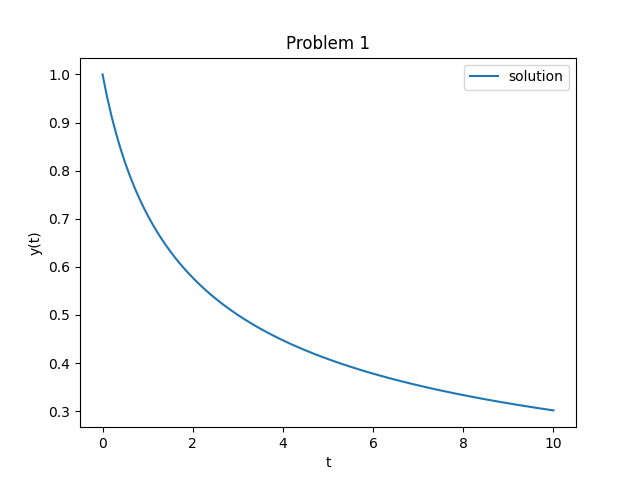
\includegraphics[width=0.7\linewidth]{./figures/solution_problem1}
\caption{Solution to the first ODE problem.}
\label{fig:solution_problem1}
\end{figure}

The second problem has the ODE:
\begin{equation}
y'(t) = \frac{y(t)(1 - \frac{y(t)}{20})}{4}.
\end{equation}
The initial condition is $y(0) = 1$ and the time domain is $[0, 10]$.

The solution to this problem is
\begin{equation}
y(t) = \frac{20e^{\frac{t}{4}}}{e^{\frac{t}{4}} + 19},
\end{equation}
as shown in Figure $\ref{fig:solution_problem2}$.

\begin{figure}[H]
\centering
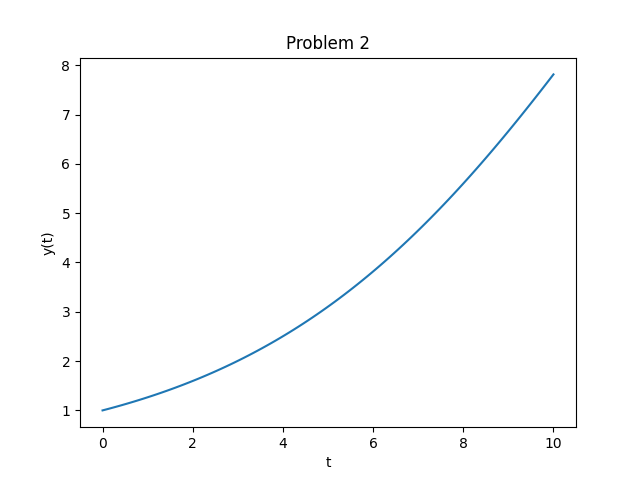
\includegraphics[width=0.7\linewidth]{./figures/solution_problem2}
\caption{Solution to the second ODE problem.}
\label{fig:solution_problem2}
\end{figure}

The third problem has the ODE:
\begin{equation}
y'(t, y) = -0.1y - e^{-0.1t}\sin(t)
\end{equation}
The initial condition is $y(0) = 1$ and the time domain is $[0, 10]$.

The solution to this problem is 
\begin{equation}
y(t) = e^{-0.1t}\cos(t),
\end{equation}
as shown in Figure $\ref{fig:solution_problem3}$.

\begin{figure}[H]
\centering
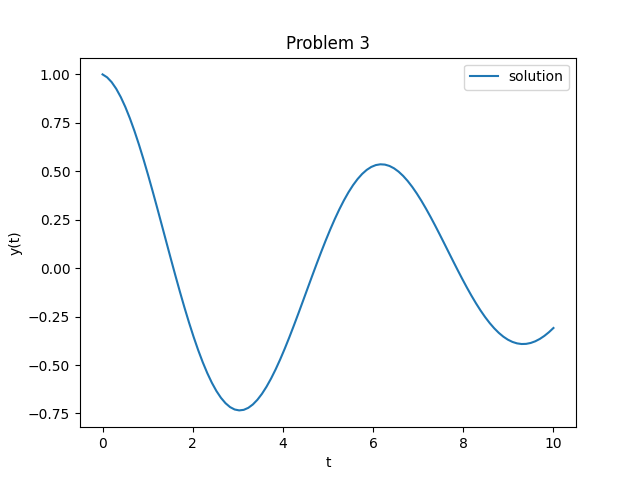
\includegraphics[width=0.7\linewidth]{./figures/solution_problem3}
\caption{Solution to the third ODE problem.}
\label{fig:solution_problem3}
\end{figure}

\subsection{Absence of control of the continuous solution approximation for typical IVODE solvers}
\label{section:end_of_step_innacurate}
In this section, we discuss how conventional solvers employed in popular packages like the Scipy library solve IVODE problems. These libraries will often have the option of using an error control solver based on a Runge-Kutta pair which works as follows. The pair comes with a low order method and a high order method and will solve an ODE by taking a sequence of steps. The solver will take each step with both methods and use the difference between the higher order method and the lower order method to generate an error estimate for the discrete numerical solution at the end of the step. If the error estimate is within the user provided tolerance, the solver will accept the step and proceed to the next step. If the error estimate is not within the tolerance, the solver will reduce the step-size and attempt to take the step again. As the error of Runge-Kutta methods depends on the step-size, a smaller step-size will produce a smaller error. The solver will keep reducing the step-size until the user tolerance is satisfied and will then proceed to the next step. In an attempt to improve the efficiency, solvers will also increase the step-size when the estimated error is significantly smaller than the tolerance.

An issue with this approach is that the error estimate is computed only for the discrete numerical solution computed at the end of a step and thus the error control is only applied at the end of the step. An interpolant that provides a continuous solution approximation across the entire step is typically constructed by the solver and it is hoped that the error of the interpolant at points within the step is within the user-provided tolerance. However, as we will show below, this is sometimes not the case.

For this interpolant to provide a solution within the user provided tolerance, the theoritical interpolation error must be less than or equal to the error of the data being fitted. Thus we would ideally use an interpolant of at least order $O(h^{p})$ if the discrete solution is of order $O(h^{p})$. However, for high order methods, it becomes too expensive to construct an interpolant of the appropriate order. IVODE solvers will thus usually compromise and employ a lower order interpolant, that is less costly, but deliver less accuracy. 

Therefore, we are not guaranteed that the continuous approximate solution is error-controlled and not guaranteed that the interpolation error will not affect the continuous solution approximation. Figures $\ref{fig:no_middle_step_error_control_p2_dop853}$ and $\ref{fig:no_middle_step_error_control_p3_rk45}$ show some results obtained when Runge-Kutta solvers are applied to some of the test problems introduced in the previous section. In these figures, we plot the global error of the numerical solution, this is the difference between the exact solution and the computed solution over the time domain. The solvers apply error control to the discrete numerical solution at the end of the step but no error control of any type to the continuous numerical solution across the step.

\begin{figure}[H]
\centering
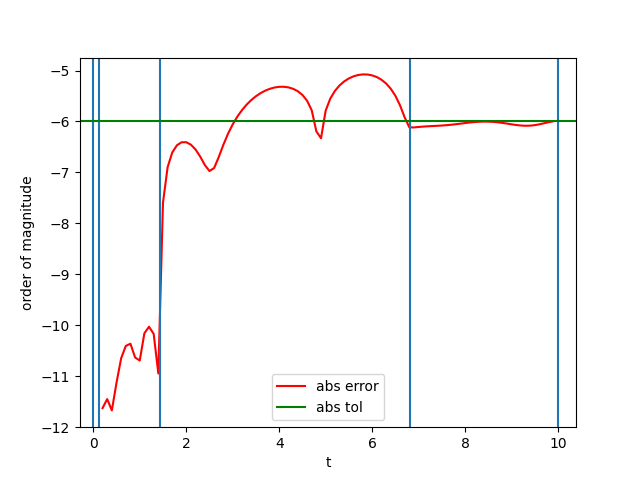
\includegraphics[width=0.7\linewidth]{./figures/no_middle_step_error_control_p2_dop853}
\caption{The Python `DOP853' solver on problem 2 with an absolute tolerance of $10^{-6}$ and a relative tolerance of $10^{-6}$. Steps are represented by the vertical lines.}
\label{fig:no_middle_step_error_control_p2_dop853}
\end{figure}

\begin{figure}[H]
\centering
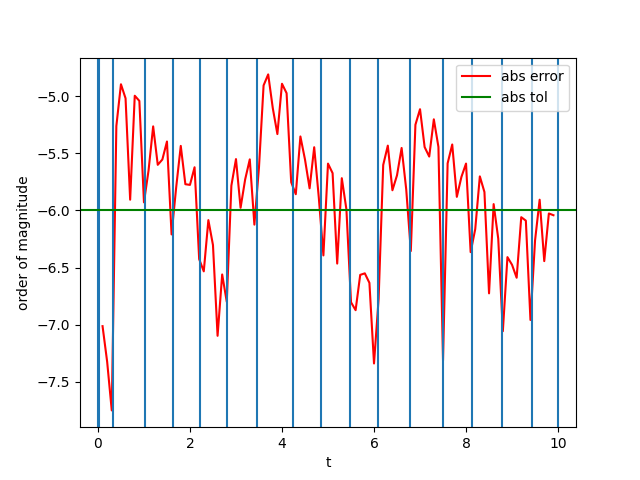
\includegraphics[width=0.7\linewidth]{./figures/no_middle_step_error_control_p3_rk45}
\caption{The Python `RK45' solver on problem 3 with an absolute tolerance of $10^{-6}$ and a relative tolerance of $10^{-6}$. Steps are represented by the vertical lines.}
\label{fig:no_middle_step_error_control_p3_rk45}
\end{figure}

Figure $\ref{fig:no_middle_step_error_control_p2_dop853}$ and $\ref{fig:no_middle_step_error_control_p3_rk45}$ shows the errors in the middle of each step obtained when applying `DOP853' to problem 2 and `RK45' to problem 3 with an absolute tolerance of $10^{-6}$ and a relative tolerance of $10^{-6}$. We can see that the solution values at the end of each step typically satisfy the tolerance. However we can clearly see that the solution values (obtained from the built-in interpolant constructed by the solver) at points within each steps, have errors up to one order of magnitude larger than the tolerance. 

We note that when a user asks for a solution whose estimated error is within a tolerance of $10^{-i}$, they expect the solution to have an estimated error that is within that tolerance for the whole time domain. However, the decision to not satisfy the user provided tolerance throughout the step is made in the interest of efficiency and the loss of accuracy in the middle of the step is the tradeoff. The goal of modern IVODE solvers is to provide a continuous solution approximation across the whole time domain. The user's expectation is that the solution approximations across each step also satisfies the tolerance as ODE solvers can be integral part of larger software packages where their approximate solutions are differentiated, integrated and manipulated in ways such that a sufficiently accurate continuous approximate solution is required. 

In this chapter, we attempt to provide an efficient way of constructing interpolants that can then be used to control the defect of the continuous approximate solution across the step and thus throughout the whole time domain.

\subsection{Defect control and the cost of traditional Continuous Runge-Kutta methods}
\label{section:crk_related_work}
In this section we introduce the `defect' of a continuous approximate solution of an ODE and explain how the control of that defect provides a type of error control of the continuous numerical solution.

In the context of numerical ODEs, the defect, denoted by $\delta(t)$,  is the amount by which the continuous numerical solution, $u(t)$, fails to satisfy the ODE. When the ODE is $y'(t) = f(t, y(t))$, the defect is 

\begin{equation}
\delta(t) = |u'(t) - f(t, u(t))|.
\end{equation}

Calculating the defect requires that the continuous approximate solution computed by the solver to also be differentiable. The idea of defect control is relatively new as differentiable solutions to ODEs can be expensive to calculate. Several investigations in this direction are outlined in \cites{MR2600928}{MR1950917}{MR1803189}{MR1239829}{MR997658}{MR996053}. In this work, the defect control method employs a continuous RK method for which the number of stages grows exponentially with the order of the method as shown in Table $\ref{tab:crk_nstages}$. In this chapter, we will compute a defect controlled continuous solution with no additional cost. A typical Runge-Kutta solver will thus be able to employ the usual number of stages required for the discrete Runge-Kutta method and still produce an accurate continuous solution.

\begin{table}[h]
\caption {Number of stages for discrete vs continuous RK method.} 
\label{tab:crk_nstages}
\begin{center}
\begin{tabular}{ c c c c} 
order   & discrete & continuous & asymptotically correct defect \\ 
4 & 4  & 4   & 8 \\ 
5 & 5  & 6   & 12 \\ 
6 & 6  & 7   & 15 \\ 
7 & 7  & 9   & 20 \\ 
8 & 8  & 13  & 27 \\ 
\end{tabular}
\end{center}
\end{table}

Though the defect is defined for the whole step, the estimation of the maximum defect within a step is what is important. If the maximum defect is within the tolerance, then the defect of the whole solution within the given step is within the tolerance. The key task is to find the location of the maximum defect within the step. One approach would be to sample the defect at several points and use the maximum value sampled. The problem with this approach is that each sampling of the defect requires an additional function evaluation. Thus we should not do too many samples. Work in this direction (cited above) involves constructing special interpolants that guarantee that (asymptotically) the maximum defect is at the same location within every step for every problem. This way only one function evaluation is required to sample the defect to obtain an estimate of the maximum defect. This is referred to as asymptotically correct defect control.

In the approach outlined in this chapter, we have observed experimentally that the maximum defect will tend to appear at one of two locations within the step. Thus in our approach, only two defect samplings must be done to get the maximum defect. Though we make an additional function evaluation compared to the asymptotically correct defect control, using no function evaluations to construct the interpolant guarantees that our method is more efficient especially for higher orders.


\subsection{Overview of our approach}
\label{section:basic_runge_kutta}
In this chapter, we will discuss simple IVODE solvers based on discrete Runge-Kutta methods of order 4, 6 and 8 and show that we can provide accurate continuous interpolant to augment the discrete solution computed by these RK methods without having to compute any additional function evaluations. In this section, we give an outline of the approach.

The first Runge-Kutta method upon which we build a prototype defect control solver is the classical $4^{th}$ order method that uses 4 stages; the second method is a Verner $6^{th}$ order method, taken from his 6(5) pair \cite{JimVernerRepo} that uses 9 stages, and the last method is a Verner $8^{th}$ order method from an 8(7) pair that uses 13 stages \cite{MR1239829}. 

The solvers that we have written use a simple step selection strategy. If the estimated maximum defect is greater than $tol$, the solver rejects the step and attempts to retake it again with half the step-size. If the estimated maximum defect is less than $0.1tol$, the solver accepts the step and doubles the step-size for the next step. We will elaborate on the initial step-size used by each solver later in the chapter.

We now note that the solver is not optimised. A more thorough analysis of how the solver behaves and thus a more refined step selection algorithm will produce a better solver in practice. The software we consider in this chapter only serves as a proof of concept for a more elaborate solver. 
\section{Time dependent discontinuity problem}
\label{section:time_problem}
In the time-dependent discontinuity problem, we change the value of the parameter $\beta$ from 0.9 to 0.005 at t=27. This introduces a discontinuity into the problem. We will show that this leads to inaccuracies in the solutions computed by the solvers, especially the fixed-step solvers. We then introduce a form of discontinuity handling, using what is known as cold starts, to show an efficient way to solve time-dependent discontinuity problems.

\subsection{Naive treatment of Covid-19 time discontinuity models}
\label{subsection:naive_time_problem}
A naive implementation of the problem is to use an if-statement inside the right-hand side function, $f(t, y)$, to implement the changes in $\beta$ as measures are implemented. An if-statement makes the function f(t, y) and its derivatives discontinuous. This introduces issues as outlined in Section $\ref{subsection:effect_of_discontinuity}$.

In pseudo code, this looks like:

\begin{minipage}{\linewidth}
\begin{lstlisting}[language=Python]
function model_with_if(t, y)
    // ...
    beta = 0.005
    if t < 27:
        beta = 0.9
    // ...
    return (dSdt, dEdt, dIdt, dRdt)
\end{lstlisting}
\end{minipage}

Also, to stay true to a naive treatment, we will always use the default tolerances in this section. Discrepancies across the programming environments that are due to tolerance issues are investigated in Section $\ref{subsection:time_tolerance_study}$.
\subsubsection{Time discontinuity model in R}

\begin{figure}[H]
\centering
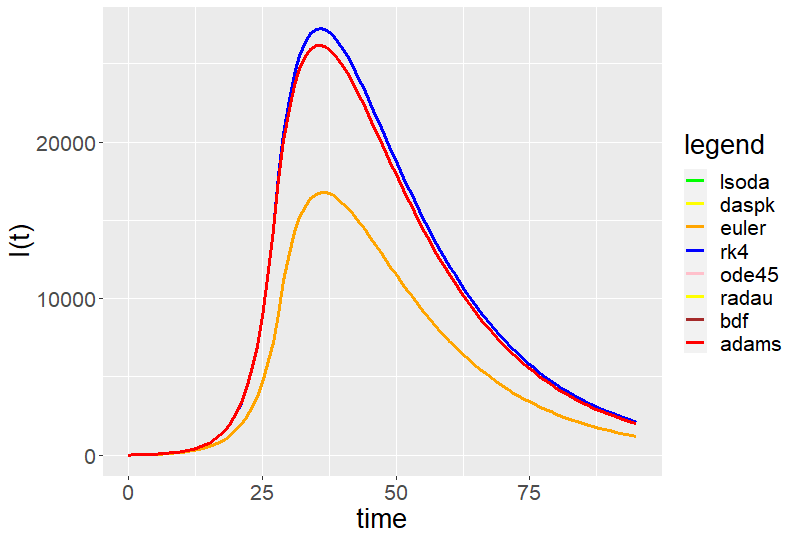
\includegraphics[width=0.7\linewidth]{./figures/time_discontinuity_R}
\caption{Solutions to the time-dependent discontinuity model using solvers from R}
\label{fig:time_discontinuity_R}
\end{figure}

From Figure $\ref{fig:time_discontinuity_R}$, we can see that all the methods except `euler' and `rk4' agree to ``eyeball" accuracy, which typically means that they agree to about two significant digits. The `rk4' method gives a solution that is somewhat close to the actual solution but the `euler' method is completely wrong. We note that all the other methods have error control while the `rk4' and `euler' methods are fixed, step-size solvers.

We also note that the `rk4' method is doing better than the `euler' method for this specific problem as it has a higher order. But the way it is performing is still better than expected. We show that this is entirely because of the issue associated with how output points are handled, as discussed in Section $\ref{subsection:solution_output_points_impl}$. If we use a bigger step-size, `rk4' gives results that just are as bad as `euler'. Figure $\ref{fig:rk4_messing_up_no_event_R}$ shows an experiment with `rk4' used with different step-sizes (space between the output points) plotted against an accurate solution in red. We can see that as soon as we change the step-size for `rk4', it does not give good results at all. Analyzing the source for `rk4' and `euler' shows that these methods select the step size using the output points requested. (The step-size is the difference between the current point and the next.) Spacing out the output points affects the step-size which affects the accuracy of the fixed step-size solver.

If a user wants to use `rk4' or `euler', to get an accurate solution, the user would have to choose a small step-size. However, the user cannot know beforehand how small a step-size is small enough to deliver a desired accuracy. Furthermore, there is the issue that a sufficiently small step-size can vary from one part of the domain to another as the problem difficulty changes. A fixed step-size solver will have to choose the smallest step required anywhere in the domain and this can lead to substantial inefficiency. A better solution is to not use fixed step-size solvers. Reputable methods with error control should be preferred as we have shown that these solvers can step over a discontinuity by resizing the step repeatedly, as needed, although this process can be very inefficient.

\begin{figure}[H]
\centering
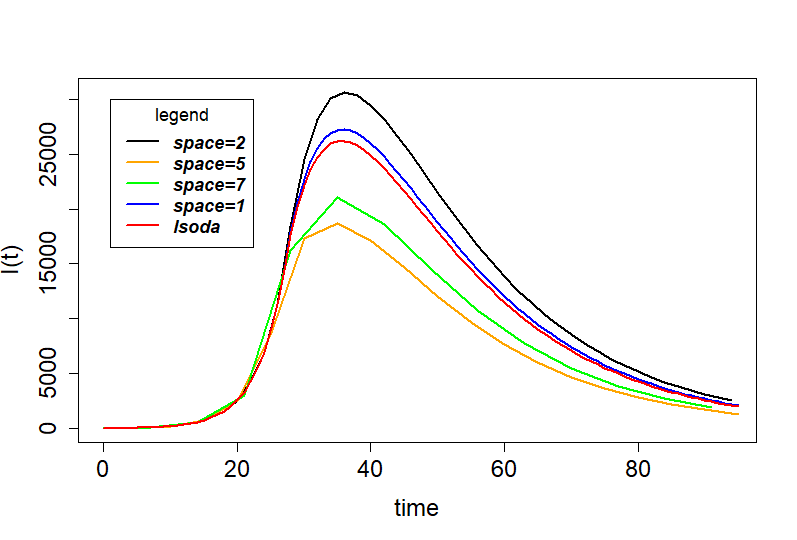
\includegraphics[width=0.7\linewidth]{./figures/rk4_messing_up_no_event_R}
\caption{Solutions computed by `rk4' in R with several fixed step-sizes compared with the accurate solution computed by LSODA}
\label{fig:rk4_messing_up_no_event_R}
\end{figure}


\subsubsection{Time discontinuity model in Python}
\begin{figure}[H]
\centering
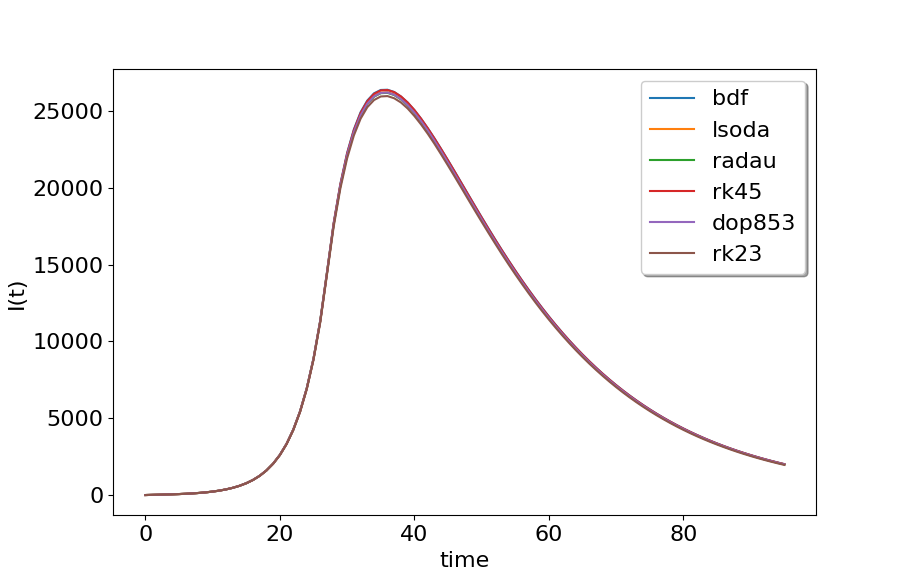
\includegraphics[width=0.7\linewidth]{./figures/time_discontinuity_py}
\caption{Solutions to the time-dependent discontinuity model using solvers from Python}
\label{fig:time_discontinuity_py}
\end{figure}
From Figure $\ref{fig:time_discontinuity_py}$, we can see that all the methods in Python's $solve\_ivp()$ work reasonably well. There is some blurring at the peak, indicating some disagreement among the methods, but all the methods provide reasonably accurate results. Python only provides error-controlled packages and thus we can see that error-control is all that is needed to step over this discontinuity. This observation also leads us to another conclusion that a reasonably sharp tolerance with an error-control method is what is required to step over this type of discontinuity. (Recall that all Python methods use a default absolute tolerance of $10^{-6}$ and a relative tolerance of $10^{-3}$.)

\subsubsection{Time discontinuity model in Scilab}
\begin{figure}[H]
\centering
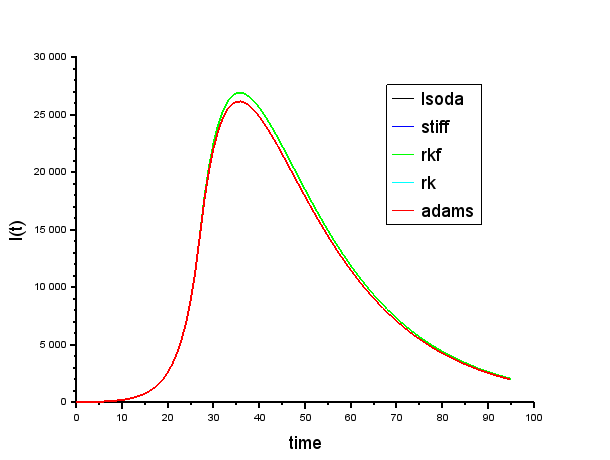
\includegraphics[width=0.7\linewidth]{./figures/time_discontinuity_scilab}
\caption{Solutions to the time-dependent discontinuity model using solvers from Scilab}
\label{fig:time_discontinuity_scilab}
\end{figure}
From Figure $\ref{fig:time_discontinuity_scilab}$, in Scilab, all the methods give similar solutions except for `rkf'. This is interesting as we know that `rkf' uses error control. This is explained by noting that `rkf' uses coarser default absolute and relative tolerances. We will show, during a tolerance analysis in Section $\ref{subsection:time_tolerance_study}$, that with a sharp enough tolerance, `rkf' also provides a reasonably accurate solution.

The other methods are all error-controlled and give similar results as expected. We note that all of the other methods have a higher default tolerance than `rkf' and thus this result is not surprising.

These results also point out that an error control solver with a sharp tolerance can step over this type of discontinuity.

\subsubsection{Time discontinuity model in Matlab}
\begin{figure}[H]
\centering
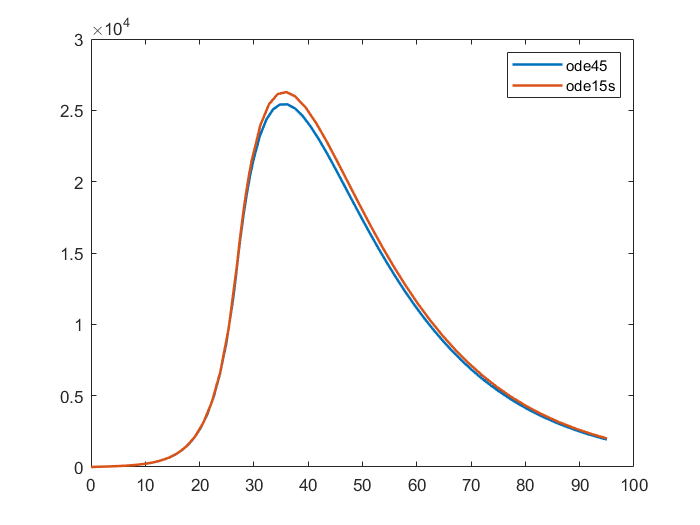
\includegraphics[width=0.7\linewidth]{./figures/time_discontinuity_matlab}
\caption{Solutions to the time-dependent discontinuity model using solvers from Matlab}
\label{fig:time_discontinuity_matlab}
\end{figure}
Figure $\ref{fig:time_discontinuity_matlab}$ shows that $ode45$ and $ode15s$ are not in agreement. This is strange because both are error controlled. We note that the same behavior of $ode45$ is seen in `rkf' in Scilab but the methods are based on different algorithms. In Matlab, both $ode45$ and $ode15s$ have the same default tolerances so we rule out that a tolerance difference is the result of this behavior. We will see that $ode45$ can give a similar result to $ode15s$ answers when the tolerance is sharp enough in Section $\ref{subsection:time_tolerance_study}$ and thus the issue may be associated with how the two solvers blend the absolute and relative tolerances.

\subsection{A better way to treat discontinuities in the time-dependent discontinuity models}
\label{subsection:time_disc_handling}
A better way to solve the time-dependent discontinuity problem is to make use of cold starts. This means that we integrate before and after the discontinuity with \emph{separate} calls to the solver. Restarting a solver with a cold start at the time of the discontinuity improves the accuracy as we will see in this and the next section. It also improves the efficiency as fewer function calls are required since we do not have the spike in function calls due to the repeated step-size resizing described in Section $\ref{subsection:effect_of_discontinuity}$.

A cold start means that we restart the solver with method parameters set so that the solver starts the computation with no values from the previous computation influencing the new integration. It will also involve using a small initial step size and for methods of varying order like the `BDF' and `Adams' methods, they will restart with the default order which is order 1.

To solve the time dependent discontinuity problem, we will integrate from time 0 to the time that measures are implemented, t=27, with one call to the solver and then use the solution values at t=27 as the initial values to make another call that will integrate (restarting with a cold start) from t=27 to $t_f$. The pseudo-code is as follows:

\begin{minipage}{\linewidth}
\begin{lstlisting}[language=Python]
initial_values = (S0, E0, I0, R0)
tspan_before = [0, 27]
solution_before = ode(intial_values, model_before_measures,
tspan_before)

initial_values_after = extract_last_row(solution_before)
tspan_after = [27, 95]
solution_after = ode(intial_values_after, 
model_after_measures, tspan_after)

solution = concatenate(solution_before, solution_after)
\end{lstlisting}
\end{minipage}

This technique can be applied to any problem where it is known when the discontinuity is introduced. This is much better than introducing a time-dependent if-statement into the model.

\subsubsection{Solving time dependent discontinuity model in R using a cold start} 
\begin{figure}[H]
\centering
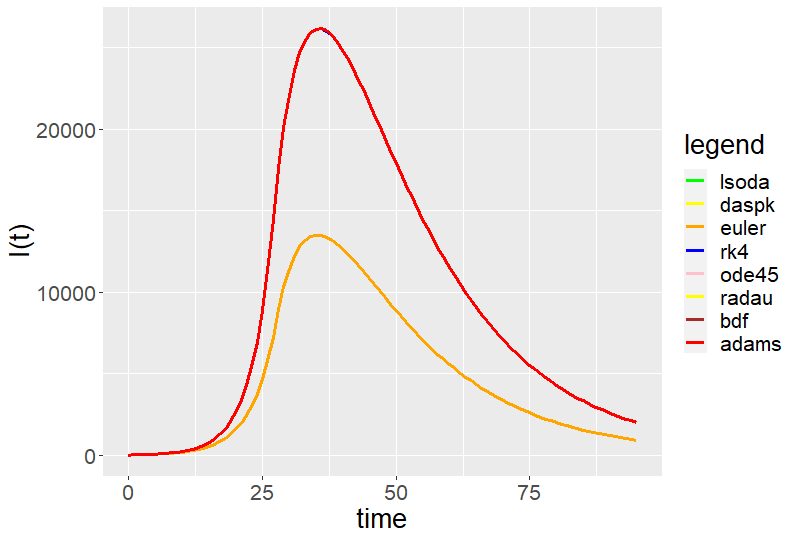
\includegraphics[width=0.7\linewidth]{./figures/solve_time_discontinuity_R}
\caption{Solutions to the time dependent discontinuity model using solvers from R and a cold start at t=27}
\label{fig:solve_time_discontinuity_R}
\end{figure}
From Figure $\ref{fig:solve_time_discontinuity_R}$, we see that the `euler' method still fails even with the cold start discontinuity handling. This is as expected as it has no error control and thus it still suffers from accuracy issues and will require smaller steps to achieve even ``eyeball" accuracy.

We see that breaking the problem into two parts makes `rk4' perform better. The method has a higher order, meaning that it does not need as small a step-size as `euler' to solve the two continuous problems but this exceptionally good performance is still unexpected. We will show in Figure $\ref{fig:rk4_messing_up_with_event_R}$ that this is only due to the use of very small step size and the performance of `rk4' is associated with the method of handling output points as described in Section $\ref{subsection:solution_output_points_impl}$.
`
\begin{figure}[H]
\centering
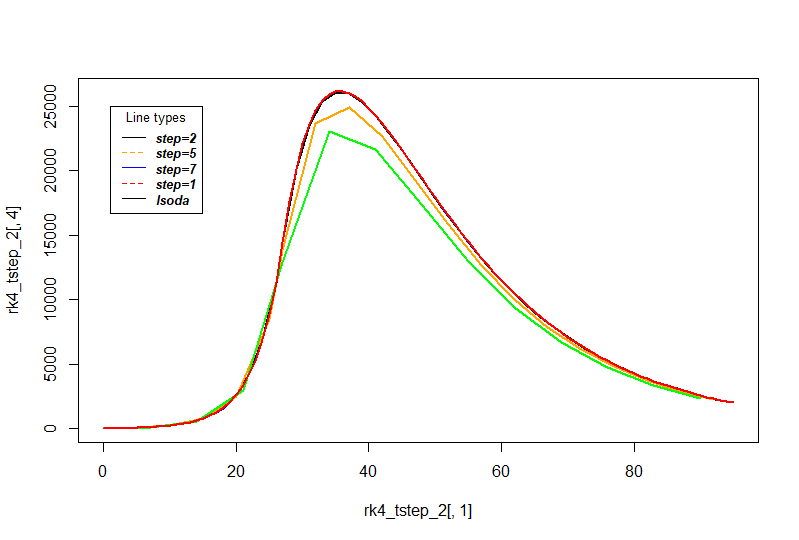
\includegraphics[width=0.7\linewidth]{./figures/rk4_messing_up_with_event_R}
\caption{The R version of `rk4' with bigger step-sizes and with discontinuity handling}
\label{fig:rk4_messing_up_with_event_R}
\end{figure}

Thus our recommendation to avoid fixed step size solvers still holds since users will not typically know how small the step size needs to be to obtain sufficient accuracy.

We also note again, that all the error-controlled solvers perform well. We will see, from the efficiency data, that using cold starts is more efficient. Using cold starts, the error control solvers do not have to step over a discontinuity and we will not have the rise in the number of function evaluations as we discussed in $\ref{subsection:effect_of_discontinuity}$. Table $\ref{tab:time_discontinuity_R}$ shows that discontinuity handling reduces the number of function evaluations. 

\begin{table}[H]
\caption {R Time Discontinuity problem efficiency data} \label{tab:time_discontinuity_R}
\begin{center}
\begin{tabular}{ c c c } 
method & no discontinuity handling & with discontinuity handling \\ 
euler & 96 & 97 \\
rk4 & 381 & 382 \\ 
lsoda & 332 & 272 \\
ode45 & 735 & 599 \\
radau & 679 & 585 \\
bdf & 423 & 263 \\
adams & 210 & 176 \\
daspk & 517 & 521
\end{tabular}
\end{center}
\end{table}

Our analysis of the efficiency data in Table $\ref{tab:time_discontinuity_R}$ starts by noting that the non-error controlled solvers in the `euler' and rk4' methods have the same number of function evaluations, the additional one being due to integrating twice at time 27. This indicates that they are just stepping from output point to output point using the same fixed step-size both with and without the discontinuity handling.

Next, we note significant decreases in the number of function evaluations for all the remaining solvers except `daspk'. These reductions in the number of function evaluations will have a significant impact on the CPU time for the difficult problem. This is entirely explained in Section $\ref{subsection:effect_of_discontinuity}$ where the error-controlled solvers have to repeatedly resize the step-size as they encounter the discontinuity.

Finally, we explain the almost constant value of the number of function evaluations for the `daspk' method through the fact that it is not using interpolation. Another experiment with a larger spacing between output points shows that it uses 627 function evaluations without discontinuity handling and 522 function evaluations with discontinuity handling.

In Section $\ref{subsection:time_tolerance_study}$, we will see that this discontinuity handling also allows us to use coarser tolerances, which improves the efficiency of the computation.

\subsubsection{Solving time dependent discontinuity model in Python using a cold start} 
\begin{figure}[H]
\centering
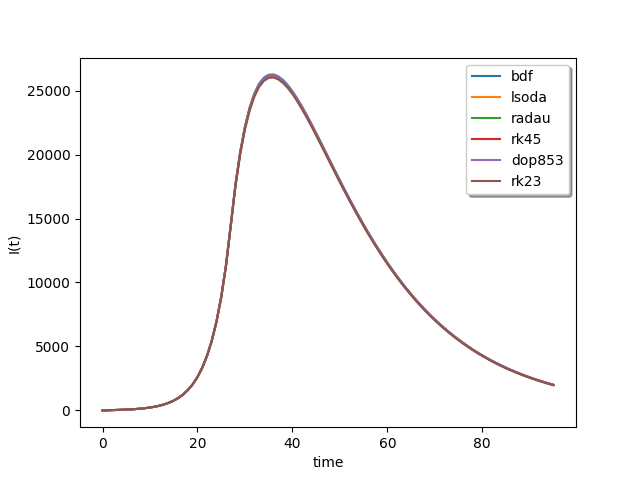
\includegraphics[width=0.7\linewidth]{./figures/solve_time_discontinuity_py}
\caption{Solutions to the time dependent discontinuity model using solvers from Python and a cold start at t=27}
\label{fig:solve_time_discontinuity_py}
\end{figure}
The Python solvers did not have significant accuracy issues even without discontinuity handling. This is because all the available methods use error control and the default tolerances are sharp enough. From Figure $\ref{fig:solve_time_discontinuity_py}$, we can see that the Python solvers again give sufficiently accurate results. Furthermore, the slight blurring at the peak has disappeared indicating that there is an even better agreement among the solvers. The addition of discontinuity handling also drastically reduces the number of function evaluations. This can be seen in Table $\ref{tab:time_discontinuity_Py}$.

\begin{table}[H]
\caption {Python Time Discontinuity problem efficiency data} \label{tab:time_discontinuity_Py} 
\begin{center}
\begin{tabular}{ c c c }
method & no discontinuity handling & with discontinuity handling \\ 
lsoda & 162 & 124 \\
rk45 & 134 & 130 \\
bdf & 202 & 146 \\
radau & 336 & 220 \\
dop853 & 329 & 181 \\
rk23 & 152 & 127 \\
\end{tabular}`
\end{center}`
\end{table}

We note that we are not using $dense\_output$ here. However, the Python solvers do not seem to allow the space between the output points to affect the accuracy. They appear to be using some form of local interpolation within each step where output is required.

From Table $\ref{tab:time_discontinuity_Py}$, we see that when discontinuity handling is introduced, the methods take fewer function evaluations. There are some huge changes for `BDF', `DOP853' and `Radau'. There are slight decreases in `LSODA' and `RK23' and only a very small decrease in `RK45'. In Section $\ref{subsection:time_tolerance_study}$, we will see that this discontinuity handling also allows us to use coarser tolerances.

\subsubsection{Solving time dependent discontinuity model in Scilab using a cold start} 
\begin{figure}[H]
\centering
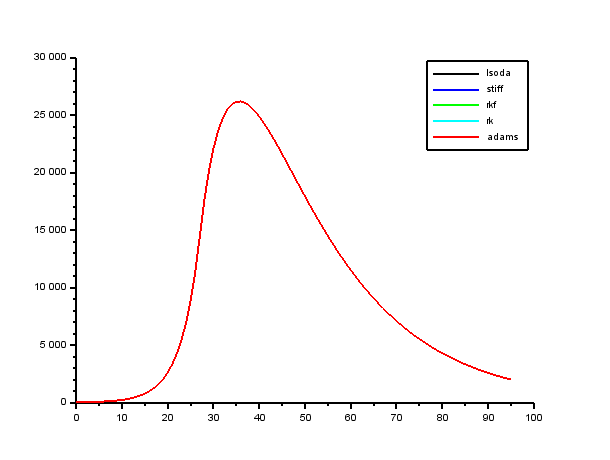
\includegraphics[width=0.7\linewidth]{./figures/solve_time_discontinuity_scilab}
\caption{Solutions to the time dependent discontinuity model using solvers from Scilab and a cold start at t=27}
\label{fig:solve_time_discontinuity_scilab}
\end{figure}
We can see from Figure $\ref{fig:solve_time_discontinuity_scilab}$ that all the methods show good agreement and thus the time-dependent discontinuity model is being solved to a reasonable accuracy. The `rkf' method is also giving reasonable results. This is despite `rkf' having a coarser default tolerance. In Section $\ref{subsection:time_tolerance_study}$, we will see that the discontinuity handling also allows us to use coarser tolerances for all solvers and thus explains why the default tolerance used by `rkf' is sufficient to allow it to solve the problem reasonably well.

The addition of discontinuity handling will also drastically reduce the number of function evaluations as seen in Table $\ref{tab:time_discontinuity_scilab}$.

\begin{table}[H]
\caption {Scilab Time Discontinuity problem efficiency data} 
\label{tab:time_discontinuity_scilab} 
\begin{center}
\begin{tabular}{ c c c }
method & no discontinuity handling & with discontinuity handling \\ 
lsoda & 346 & 292 \\
stiff & 531 & 362 \\
rkf & 589 & 590 \\
rk & 1649 & 1473 \\
adams & 304 & 221 \\
\end{tabular}
\end{center}
\end{table}

From Table $\ref{tab:time_discontinuity_scilab}$, we see that all the methods use fewer function evaluations. We see substantial decreases in the number of function evaluations for `lsoda', `stiff', `rk' and `adams'.`

The odd function value counts for `rkf' (the number of function evaluations does not decrease) occurs because `rkf' is using the method for handling output points as outlined in Section $\ref{subsection:solution_output_points_impl}$. The results, when we space out the output points more, are 335 function evaluations without discontinuity handling and 292 function evaluations with discontinuity handling.

We note that the high number of function evaluations in `rk' with and without discontinuity handling is because it is using Richardson extrapolation to get an error estimate. Richardson involves using the Runge-Kutta method twice, once to get the solution and once again with half the step-size to do two steps in the same interval to get a more accurate solution to use to obtain an error estimate. Thus in one actual step, there are three `steps' and this leads to a large number of function evaluations.

\subsubsection{Solving time dependent discontinuity model in Matlab using a cold start}
\begin{figure}[H]
\centering
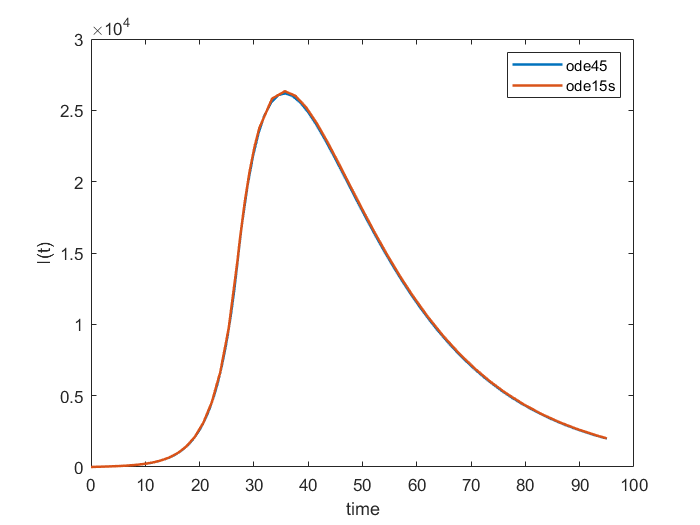
\includegraphics[width=0.7\linewidth]{./figures/solve_time_discontinuity_matlab}
\caption{Solutions to the time dependent discontinuity model using solvers from Matlab and a cold start at t=27}
\label{fig:solve_time_discontinuity_matlab}
\end{figure}

From Figure $\ref{fig:solve_time_discontinuity_matlab}$ we can see that both solvers give similar solutions. We remember that with an if-statement inside the function $f(t, y(t))$ that the two solvers gave different solutions. As we will show in Section $\ref{subsection:time_tolerance_study}$, the discontinuity handling allows us to use a coarser tolerance and thus allows $ode45$ to give a reasonably accurate result.

We also show in Table $\ref{tab:time_discontinuity_matlab}$ that discontinuity handling allows the solvers to use fewer function evaluations.

\begin{table}[H]
\caption {Matlab Time Discontinuity problem efficiency data} 
\label{tab:time_discontinuity_matlab} 
\begin{center}
\begin{tabular}{ c c c }
method & no discontinuity handling & with discontinuity handling \\ 
ode45 & 175 & 164 \\
ode15s & 144 & 113 \\
\end{tabular}
\end{center}
\end{table}

From Table $\ref{tab:time_discontinuity_matlab}$, $ode45$ uses 11 less function evaluations while $ode15s$ uses 31 less function evaluations.

\subsection{Efficiency data and tolerance study for the time discontinuous problem}
\label{subsection:time_tolerance_study}
It is not uncommon for researchers to use an ODE solver in a loop or within an optimization algorithm so that they can study models with different problem-dependent parameters. In such contexts, it may be reasonable to coarsen the tolerances whenever the computation is taking too long. In this section, we investigate how coarse we can set the tolerance while still obtaining reasonably accurate results for the time-dependent discontinuity model. 

We investigate `lsoda' across R, Python, and Scilab as they all appear to use the same source code. We use this experiment to show that discontinuity handling allows us to use coarser tolerances.

We will also investigate `rkf' in Scilab as it has a smaller default tolerance than the other Scilab solvers, and $ode45()$ in Matlab, both of which failed to solve the time-dependent discontinuity model. We will show that they can solve the problem without discontinuity handling only at sharper tolerances than the default tolerances. We also investigate solvers based on Runge-Kutta pairs of the same order as the pair used in `rkf' and $ode45$ in the other programming environments; R and Python have a version of DOPRI5 but do not share the same source code. The DOPRI5 in Python is a Python implementation and the one in R is an interface to a C implementation. $ode45$ in Matlab uses DOPRI5 but it is implemented in the Matlab programming language.

\subsubsection{Comparing LSODA across platforms for time discontinuous problem}
\subparagraph{Time discontinuity LSODA tolerance study in R}
In this section, we run the R LSODA solver with multiple tolerances with and without discontinuity handling. We will set both the relative and absolute tolerances to various values and see how coarse we can keep the tolerance while still obtaining reasonably accurate results. We also look at efficiency data to observe decreases in the number of function evaluations.

\begin{figure}[H]
\centering
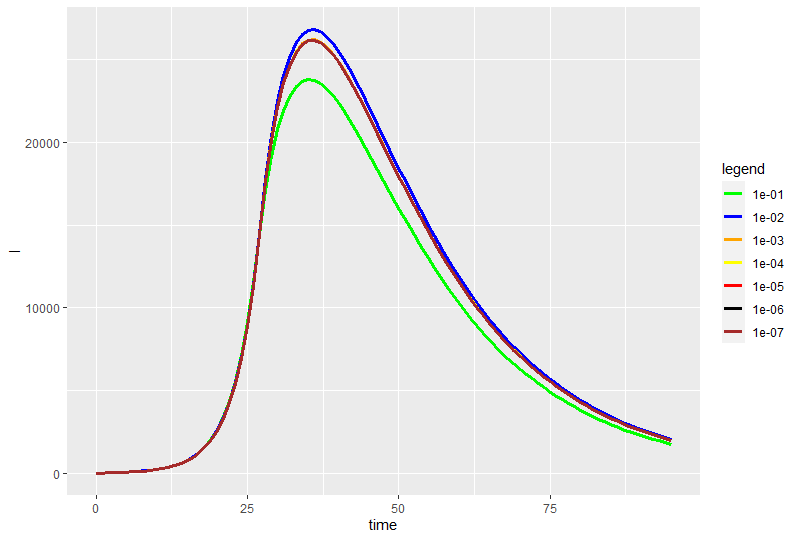
\includegraphics[width=0.7\linewidth]{./figures/tolerance_time_lsoda_no_event_R}
\caption{Time discontinuity model tolerance study on the R version of LSODA without a cold start}
\label{fig:tolerance_time_lsoda_no_event_R}
\end{figure}

\begin{figure}[H]
\centering
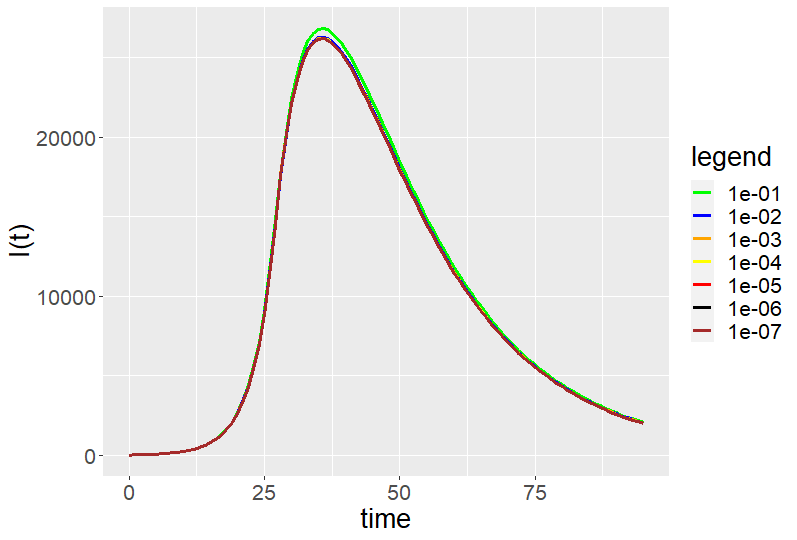
\includegraphics[width=0.7\linewidth]{./figures/tolerance_time_lsoda_with_event_R}
\caption{Time discontinuity model tolerance study on the R version of LSODA with a cold start}
\label{fig:tolerance_time_lsoda_with_event_R}
\end{figure}

From Figures $\ref{fig:tolerance_time_lsoda_no_event_R}$ and $\ref{fig:tolerance_time_lsoda_with_event_R}$, we can see that the addition of discontinuity handling allows the solver to use coarser tolerances and still get a reasonable result; we need a tolerance of $10^{-3}$ and sharper tolerances without discontinuity handling but can use a tolerance of $10^{-2}$ and sharper with it. This supports the observation that the use of discontinuity handling when solving a discontinuous problem. Also, using coarser tolerances gives us more efficiency, as we will see in Table $\ref{tab:tolerance_time_discontinuity_lsoda_R}$. 

\begin{table}[H]
\caption {R LSODA time Discontinuity tolerance study} \label{tab:tolerance_time_discontinuity_lsoda_R} 
\begin{center}
\begin{tabular}{ c c c }
tolerance & no discontinuity handling & with discontinuity handling \\ 
1e-01 & 197 & 200 \\
1e-02 & 214 & 206 \\
1e-03 & 264 & 212 \\
1e-04 & 264 & 224 \\
1e-05 & 317 & 244 \\
1e-06 & 332 & 272 \\
1e-07 & 393 & 298 \\
\end{tabular}
\end{center}
\end{table}

From Table $\ref{tab:tolerance_time_discontinuity_lsoda_R}$, we see that for the coarser tolerances, the number of function evaluations is roughly the same. But with sharper tolerances, a lot more function evaluations are required and thus if we had a user-provided function that was expensive to evaluate, we would see clear reductions in computation times.

A similar number of function evaluations for the coarser tolerances should not distract us from the fact that the solver without discontinuity handling at these tolerances gives results that are not as accurate as the results obtained using the solver with discontinuity handling. The small differences of 3 function evaluations for the 0.1 tolerance case and 8 function evaluations in the 0.01 case do not excuse the fact that the solutions are significantly less accurate.

\subparagraph{Time discontinuity LSODA tolerance study in Python}
In this section, we run the Python version of the LSODA solver with multiple tolerances with and without discontinuity handling. We note that the Python solvers were giving sufficiently accurate results in both cases apart from some small disagreements in the case where no discontinuity handling is employed but we will see how coarse we can choose the tolerance while still obtaining reasonably accurate results. We set both the relative and absolute tolerances to various values. We also look at efficiency data to see the decreases in the number of function evaluations.

\begin{figure}[H]
\centering
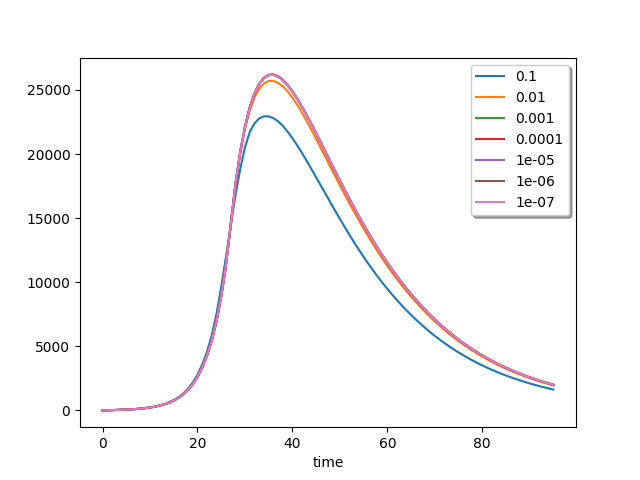
\includegraphics[width=0.7\linewidth]{./figures/tolerance_time_lsoda_no_event_py}
\caption{Time discontinuity model tolerance study on the Python version of LSODA without a cold start}
\label{fig:tolerance_time_lsoda_no_event_py}
\end{figure}

\begin{figure}[H]
\centering
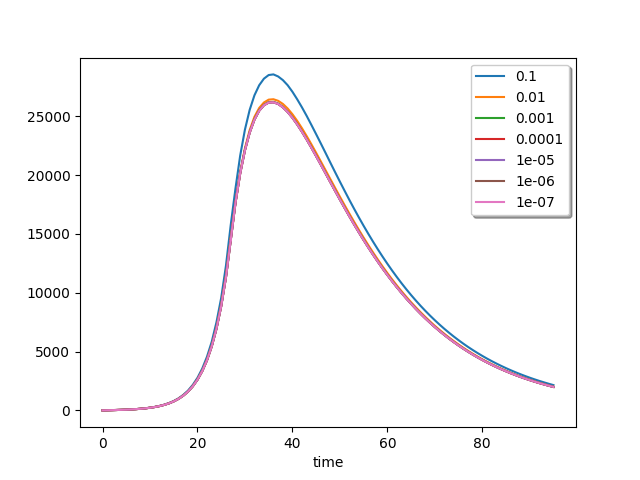
\includegraphics[width=0.7\linewidth]{./figures/tolerance_time_lsoda_with_event_py}
\caption{Time discontinuity model tolerance study on the Python version of LSODA with a cold start}
\label{fig:tolerance_time_lsoda_with_event_py}
\end{figure}

From Figures $\ref{fig:tolerance_time_lsoda_with_event_py}$ and $\ref{fig:tolerance_time_lsoda_no_event_py}$, we see that the use of the discontinuity handling lets us use a coarser tolerance since a tolerance of $10^{-2}$ was enough to get a reasonably accurate result with the discontinuity handling whereas a tolerance of $10^{-3}$ was needed otherwise. This tells us that using discontinuity handling will improve our results for a more complex time-dependent discontinuity problem.

In turn, the use of coarser tolerances give us more efficiency. (See Table $\ref{tab:tolerance_time_discontinuity_lsoda_py}$.)

\begin{table}[H]
\caption {Python LSODA Time Discontinuity tolerance study} \label{tab:tolerance_time_discontinuity_lsoda_py} 
\begin{center}
\begin{tabular}{ c c c }
tolerance & no discontinuity handling & with discontinuity handling \\ 
0.1 & 79 & 86 \\
0.01 & 98 & 93 \\
0.001 & 156 & 116 \\
0.0001 & 185 & 146 \\
1e-05 & 259 & 186 \\
1e-06 & 283 & 228 \\
1e-07 & 361 & 272 \\
\end{tabular}
\end{center}
\end{table}
Again, in Table $\ref{tab:tolerance_time_discontinuity_lsoda_py}$, we see that that at coarse tolerances, the number of function evaluations is roughly the same. This similar number of function evaluations does not excuse the fact that the coarser tolerances are giving erroneous solutions when discontinuity handling is not employed.

At sharper tolerances, where the comparison is fair, the number of function evaluations is much smaller with discontinuity handling than without; we make 40 fewer function evaluations at 0.001 and 0.0001 and we do many fewer function evaluations for sharper tolerances. We note that if the function for the evaluation of the right-hand side of the ODE was more time-consuming, this reduced number of function evaluations will cause a significant decrease in the CPU times.

\subparagraph{Time discontinuity LSODA tolerance study in Scilab}
In this section, we run the Scilab version of the LSODA solver with multiple tolerances with and without discontinuity handling. We will set both the relative and absolute tolerances to various values and see how coarse we can set the tolerance while still getting reasonably accurate results.

\begin{figure}[H]
\centering
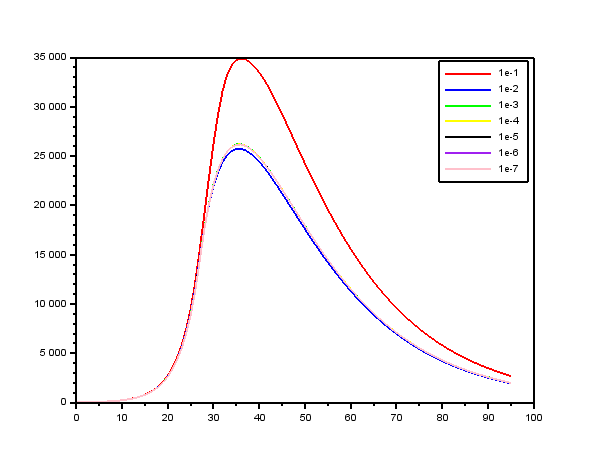
\includegraphics[width=0.7\linewidth]{./figures/tolerance_time_lsoda_no_event_sci}
\caption{Time discontinuity model tolerance study on the Scilab version of lsoda without a cold start}
\label{fig:tolerance_time_lsoda_no_event_sci}
\end{figure}

\begin{figure}[H]
\centering
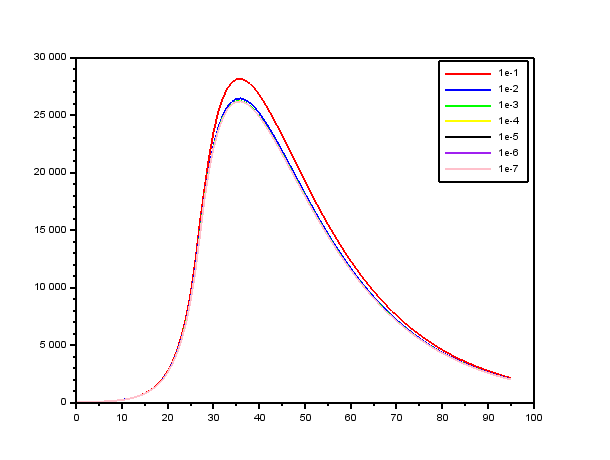
\includegraphics[width=0.7\linewidth]{./figures/tolerance_time_lsoda_with_event_sci}
\caption{Time discontinuity model tolerance study on the Scilab version of lsoda with a cold start}
\label{fig:tolerance_time_lsoda_with_event_sci}
\end{figure}

From Figures $\ref{fig:tolerance_time_lsoda_no_event_sci}$ and $\ref{fig:tolerance_time_lsoda_with_event_sci}$ we can see that for tolerances from $10^{-1}$ to $10^{-4}$, the Scilab version of LSODA without discontinuity handling fails but we are able to use a tolerance as coarse as $10^{-2}$ with discontinuity handling. 

It is interesting to see how far off the solution without discontinuity handling is at a tolerance of $10^{-1}$. We also note that this behavior is different from the R and the Python version LSODA but this may be due to the way Scilab handles the tolerances.

\begin{table}[H]
\caption {Scilab LSODA Time Discontinuity tolerance study} 
\label{tab:tolerance_time_discontinuity_lsoda_scilab} 
\begin{center}
\begin{tabular}{ c c c }
tolerance & no discontinuity handling & with discontinuity handling \\ 
0.1 & 80 & 82 \\
0.01 & 98 & 92 \\
0.001 & 156 & 116 \\
1e-4 & 185 & 146 \\
1e-5 & 255 & 186 \\
1e-6 & 280 & 228 \\
1e-7 & 361 & 272 \\
\end{tabular}
\end{center}
\end{table}
Again, in Table $\ref{tab:tolerance_time_discontinuity_lsoda_scilab}$, we see that the number of function evaluations is roughly the same at coarser tolerances but that at sharp tolerances, where both types of computations give reasonably accurate solutions and thus allow for a fair comparison, the solver with discontinuity handling performs better than the solver without discontinuity handling. We can use up to 90 fewer function evaluations through the use of discontinuity handling. 

\subsubsection{Comparing solvers based on Runge-Kutta pairs across platforms for the time discontinuous problem}
\subparagraph{Time discontinuity tolerance study on the R version of DOPRI5}
In this section, we use the R version of DOPRI5, which is the `ode45' method of the $ode()$ function, with multiple tolerances with and without discontinuity handling. We will set both the relative and absolute tolerances to various values and see how coarse we can choose the tolerance while still getting reasonably accurate results. We also look at efficiency data to see the decreases in the number of function evaluations when discontinuity handling is employed.

\begin{figure}[H]
\centering
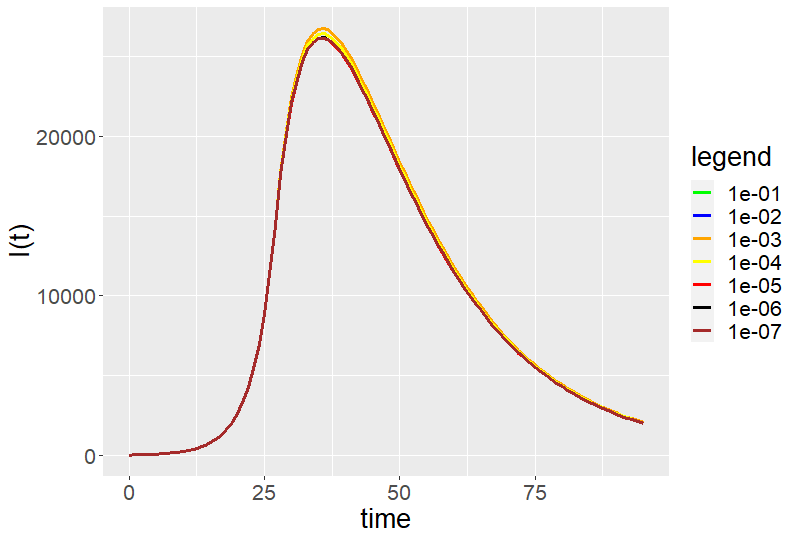
\includegraphics[width=0.7\linewidth]{./figures/tolerance_time_rk45_no_event_R}
\caption{Time Discontinuity model tolerance study on the R version of DOPRI5 without discontinuity handling}
\label{fig:tolerance_time_rk45_no_event_R}
\end{figure}

\begin{figure}[H]
\centering
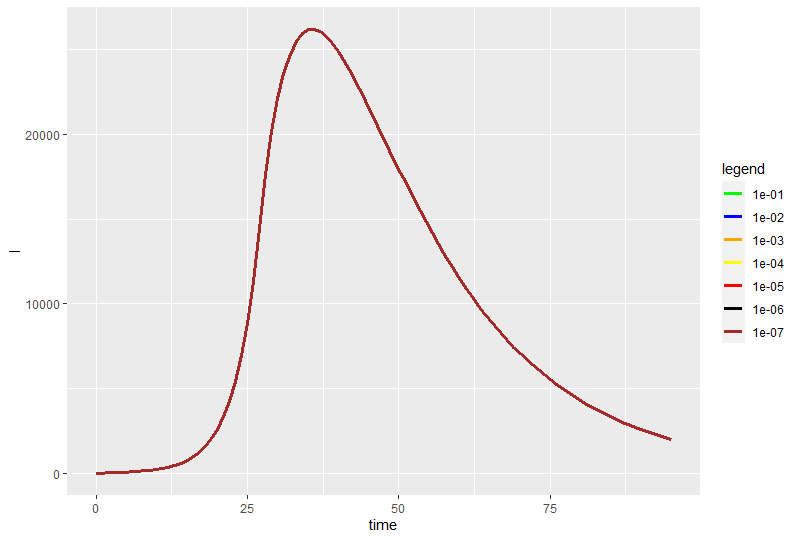
\includegraphics[width=0.7\linewidth]{./figures/tolerance_time_rk45_with_event_R}
\caption{Time Discontinuity model tolerance study on the R version of DOPRI5 with discontinuity handling}
\label{fig:tolerance_time_rk45_with_event_R}
\end{figure}

From Figures $\ref{fig:tolerance_time_rk45_no_event_R}$ and $\ref{fig:tolerance_time_rk45_with_event_R}$, we see that the addition of discontinuity handling lets us use a coarser tolerance and still get a reasonably accurate answer. Without discontinuity handling, we had to use $10^{-4}$ for both the absolute and relative tolerance but with discontinuity handling, we can use $10^{-1}$. 

However, as we will see in the Python version of DOPRI5, the results from Figures $\ref{fig:tolerance_time_rk45_no_event_R}$ and $\ref{fig:tolerance_time_rk45_with_event_R}$ are suspicious and stem from the fact that R is not using a proper interpolation scheme to produce the results. It is using an algorithm for interpolation that depends on the selected output points and which affects efficiency and accuracy, as discussed in Section $\ref{subsection:solution_output_points_impl}$. 

\begin{table}[H]
\caption {R DOPRI5 Time Discontinuity tolerance study} \label{tab:tolerance_time_discontinuity_rk45_R} 
\begin{center}
\begin{tabular}{ c c c }
tolerance & no discontinuity handling & with discontinuity handling\\ 
1e-01 & 572 & 574 \\
1e-02 & 572 & 574 \\
1e-03 & 572 & 574 \\
1e-04 & 612 & 574 \\
1e-05 & 692 & 587 \\
1e-06 & 735 & 599 \\
1e-07 & 926 & 702 \\
\end{tabular}
\end{center}
\end{table}

Table $\ref{tab:tolerance_time_discontinuity_rk45_R}$ also confirms our suspicions since, at coarser tolerances, $10^{-1}$ to $10^{-3}$, the number of function evaluations does not change at all. This indicates that something else, not the tolerance nor the discontinuity, is the limiting factor for the number of function evaluations and that this other factor leads to a need for around 572 or 574 function evaluations.

We suspect that the R DOPRI5 version is not using interpolation or some other dense output technique to produce its solutions and that it is integrating using the output points to determine the step-size. We therefore will do the following experiment where we specify a smaller set of output points with the points further spaced out from each other.

\begin{figure}[H]
\centering
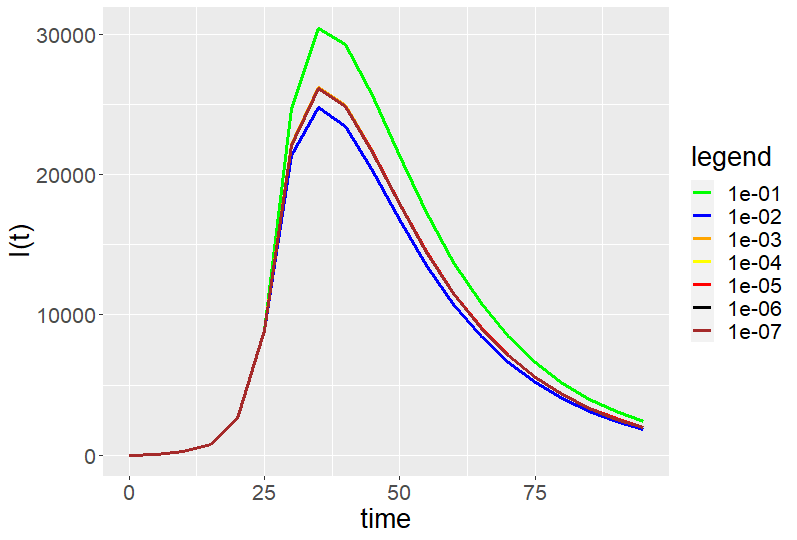
\includegraphics[width=0.7\linewidth]{./figures/tolerance_time_rk45_further_no_event_R}
\caption{Time Discontinuity model tolerance study on the R version of DOPRI5 without discontinuity handling and output points more spaced out}
\label{fig:tolerance_time_rk45_further_no_event_R}
\end{figure}

\begin{figure}[H]
\centering
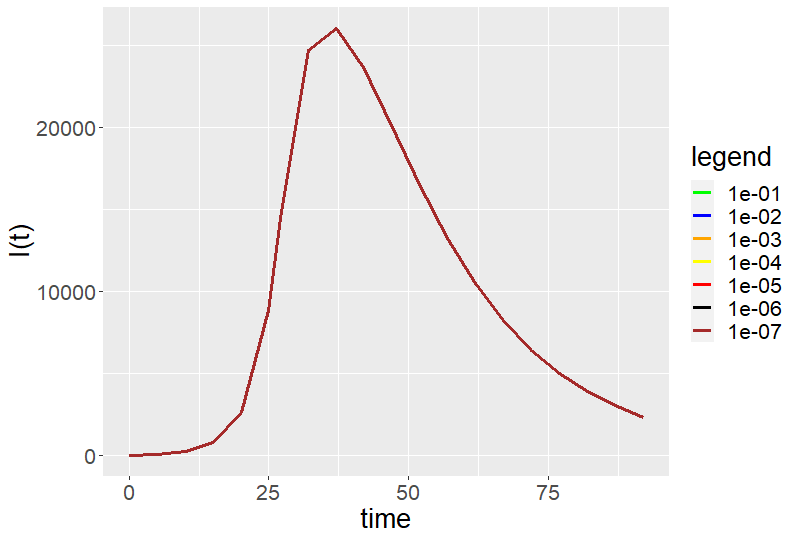
\includegraphics[width=0.7\linewidth]{./figures/tolerance_time_rk45_further_with_event_R}
\caption{Time Discontinuity model tolerance study on the R version of DOPRI5 with discontinuity handling and output points more spaced out}
\label{fig:tolerance_time_rk45_further_with_event_R}
\end{figure}

From Figures $\ref{fig:tolerance_time_rk45_further_no_event_R}$ and $\ref{fig:tolerance_time_rk45_further_with_event_R}$, we can now see a more drastic change in the solution when the output points are further spaced out. Also, we see in Table $\ref{tab:tolerance_time_discontinuity_rk45_further_R}$ that the number of function evaluations actually changes with the tolerance.

Using these two figures, we also see that discontinuity handling is allowing us to use coarser tolerances. We can use even a tolerance of $10^{-1}$ with discontinuity handling while getting a reasonably accurate result, whereas, without discontinuity handling, we need to use a tolerance of $10^{-3}$ or sharper tolerances to get a reasonably accurate answer.

\begin{table}[H]
\caption {R DOPRI5 Time Discontinuity tolerance study with spaced output points} \label{tab:tolerance_time_discontinuity_rk45_further_R} 
\begin{center}
\begin{tabular}{ c c c }
tolerance & no discontinuity handling & with discontinuity handling \\ 
1e-01 & 116 & 112 \\
1e-02 & 142 & 125 \\
1e-03 & 168 & 131 \\
1e-04 & 246 & 162 \\
1e-05 & 352 & 235 \\
1e-06 & 614 & 349 \\
1e-07 & 796 & 542 \\
\end{tabular}
\end{center}
\end{table}

Our analysis of Table $\ref{tab:tolerance_time_discontinuity_rk45_further_R}$ begins by noting that the set of output points is no longer a limiting factor. We can see the number of function evaluations change with the tolerance now and this indicates that the tolerance is controlling the step-size. This confirms our suspicions that the R implementation of DOPRI5 is not using a proper interpolation scheme. Instead, it is allowing the vector of desired output points which its interface uses dictate the efficiency of the solver.

Regarding the accuracy of the solver as we coarsen the tolerance we can see from Figures $\ref{fig:tolerance_time_rk45_further_no_event_R}$ and $\ref{fig:tolerance_time_rk45_further_with_event_R}$ that even at a tolerance of $10^{-1}$, the solver with the discontinuity handling is still able to produce reasonably accurate solutions whereas it requires a tolerance of $10^{-3}$ for the solver without the discontinuity handling.

The new table, Table $\ref{tab:tolerance_time_discontinuity_rk45_further_R}$, does offer some more insights. Again we can see that at coarser tolerances, the decrease in the number of function evaluations is small but as the tolerance is sharpened, the number of function evaluations decreases significantly. The relatively similar number of function evaluations at the coarser tolerances does not excuse the fact that the solver without discontinuity handling is not getting a reasonably accurate answer. 

\subparagraph{Time discontinuity model tolerance study on Python's version of DOPRI5}
In this section, we run Python's version of DOPRI5, which is aliased under 'RK45' from the $solver\_ivp()$ function, with multiple tolerances with and without discontinuity handling. We will set both the relative and absolute tolerances to various values and see how coarse we can choose the tolerance while still obtaining reasonable accurate results. We also look at efficiency data to see the decreases in the number of function evaluations.

\begin{figure}[H]
\centering
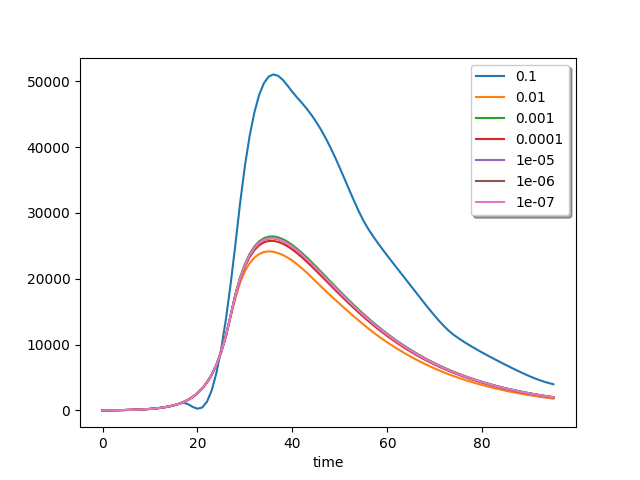
\includegraphics[width=0.7\linewidth]{./figures/tolerance_time_rk45_no_event_py}
\caption{Time Discontinuity model tolerance study on the Python version of DOPRI5 without discontinuity handling}
\label{fig:tolerance_time_rk45_no_event_py}
\end{figure}

\begin{figure}[H]
\centering
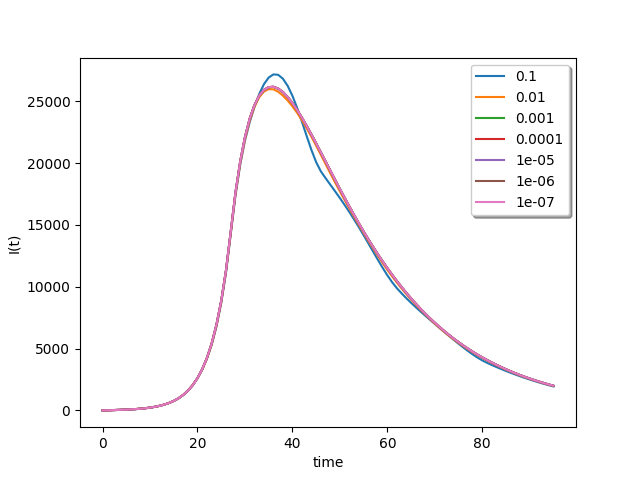
\includegraphics[width=0.7\linewidth]{./figures/tolerance_time_rk45_with_event_py}
\caption{Time Discontinuity model tolerance study on the Python version of DOPRI5 with discontinuity handling}
\label{fig:tolerance_time_rk45_with_event_py}
\end{figure}

From Figures $\ref{fig:tolerance_time_rk45_with_event_py}$ and $\ref{fig:tolerance_time_rk45_no_event_py}$, we can see clear differences at the different tolerance values. This is in contrast with the first tolerance study on the R version of DOPRI5. From studying Python's $solve\_ivp$ interface and source code, we note that Python is using dense output/interpolation. We can explain the R version of DOPRI5 performance entirely because it does not use interpolation by default but instead stops at every output point.

We then compare the Python version of DOPRI5 with and without discontinuity handling. We can see that the use of discontinuity handling allows us to use coarser tolerances in Python while obtaining reasonably accurate results. We see that we need a tolerance of $10^{-5}$ or sharper to get reasonably accurate solutions without discontinuity handling while a tolerance of $10^{-2}$ is small enough when discontinuity handling is employed. We will also see in Table $\ref{tab:tolerance_time_discontinuity_rk45_py}$ that the solver with discontinuity handling is much more efficient.


\begin{table}[H]
\caption {Python DOPRI5 Time Discontinuity tolerance study} \label{tab:tolerance_time_discontinuity_rk45_py} 
\begin{center}
\begin{tabular}{ c c c }
tolerance & no discontinuity handling & with discontinuity handling \\ 
0.1 & 68 & 70 \\
0.01 & 86 & 88 \\
0.001 & 146 & 124 \\
0.0001& 224 & 172 \\
1e-05 & 326 & 250 \\
1e-06 & 488 & 370 \\
1e-07 & 752 & 568 \\
\end{tabular}
\end{center}
\end{table}

From Table $\ref{tab:tolerance_time_discontinuity_rk45_py}$, we see that at coarser tolerances, the number of function evaluations is lower with the discontinuity handling than without discontinuity handling. We should also point out that in Python, DOPRI5 at coarse tolerances gives very inaccurate results, the errors are too large to excuse the small gain in efficiency.

At sharper tolerances where we get reasonably accurate results both with and without discontinuity handling, and thus a fair comparison can be done, we can see that the code with discontinuity handling performs much better. At a tolerance of $10^{-7}$, the drop in the number of function evaluations is very significant and would lead to much faster execution times, whereas for a tolerance of $10^{-5}$ or sharper, the decrease in the number of function evaluations is 75 or more.

\subparagraph{Time discontinuity model tolerance study on the Scilab version of RKF45}
In this section, we run the Scilab version of RKF45 aliased as `rkf' in the $ode()$ function with different tolerances. We note that the default tolerance for the Scilab `rkf' function was not enough to solve the problem to reasonable accuracy without discontinuity handling but using cold starts did solve the problem even with that default tolerance. 

By running `rkf' at various tolerances, we will show that it can also compute with reasonably accurate solutions at sharper tolerances without discontinuity handling. Thus the anomaly we saw in Section $\ref{subsection:naive_time_problem}$ occurred entirely because the solver has a coarser default tolerance than the other methods.

We will also see that using discontinuity handling lets us use fewer function evaluations which, given a more complex problem, will result in a significant improvement in computation times.

\begin{figure}[H]
\centering
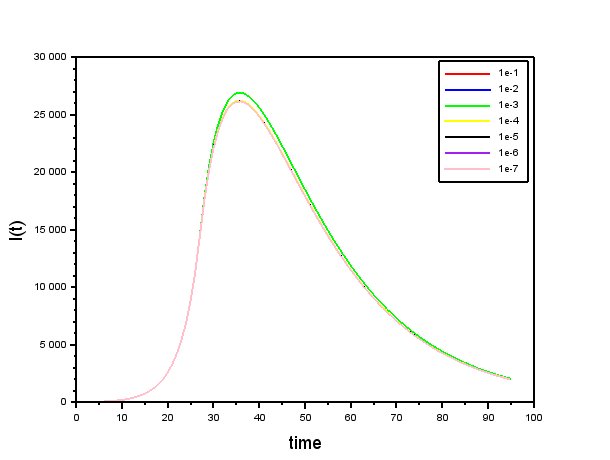
\includegraphics[width=0.7\linewidth]{./figures/tolerance_time_rk45_no_event_sci}
\caption{Time discontinuity model tolerance study on the Scilab version of RKF45 without discontinuity handling}
\label{fig:tolerance_time_rk45_no_event_sci}
\end{figure}

\begin{figure}[H]
\centering
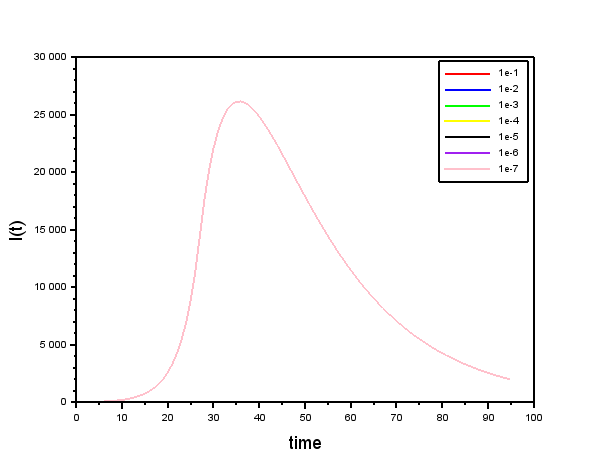
\includegraphics[width=0.7\linewidth]{./figures/tolerance_time_rk45_with_event_sci}
\caption{Time discontinuity model tolerance study on the Scilab version of RKF45 with discontinuity handling}
\label{fig:tolerance_time_rk45_with_event_sci}
\end{figure}

We see from Figure $\ref{fig:tolerance_time_rk45_no_event_sci}$ that using $10^{-4}$ for both the absolute and the relative tolerance gives reasonably accurate answers and that anything coarser does not work. We then remember that the relative tolerance defaults to $10^{-3}$ and the absolute tolerance defaults to $10^{-4}$ for `rkf' which is slightly coarser than what is needed to get a reasonably accurate solution.

Figure $\ref{fig:tolerance_time_rk45_with_event_sci}$ is also interesting as it seems to indicate that a tolerance of $10^{-1}$ is enough to get the correct solution with discontinuity handling. This is surprising but consistent with our observations for R and Python Runge-Kutta pairs.

\begin{table}[H]
\caption {Scilab RKF45 Time Discontinuity tolerance study} 
\label{tab:tolerance_time_discontinuity_rk45_scilab} 
\begin{center}
\begin{tabular}{ c c c }
tolerance & no discontinuity handling & with discontinuity handling\\ 
0.1 & 577 & 584 \\
0.01 & 577 & 584 \\
0.001 & 583 & 584 \\
1e-4 & 641 & 590 \\
1e-5 & 674 & 608 \\
1e-6 & 847 & 764 \\
1e-7 & 924 & 830 \\
\end{tabular}
\end{center}
\end{table}
We can see from Table $\ref{tab:tolerance_time_discontinuity_rk45_scilab}$ that the Scilab `rkf' method is not using interpolation. We can say this because even at extremely low tolerances, it is still using the same number of function evaluations. There is also no difference with and without discontinuity handling. We also note that the tolerance did not change the number of function evaluations and thus something else is determining the number of function evaluations. Doing the same experiment with the points further spaced out shows us that it is the spacing of the output points that is causing the issue.

We start by replicating the experiments in the previous sections.
\begin{figure}[H]
\centering
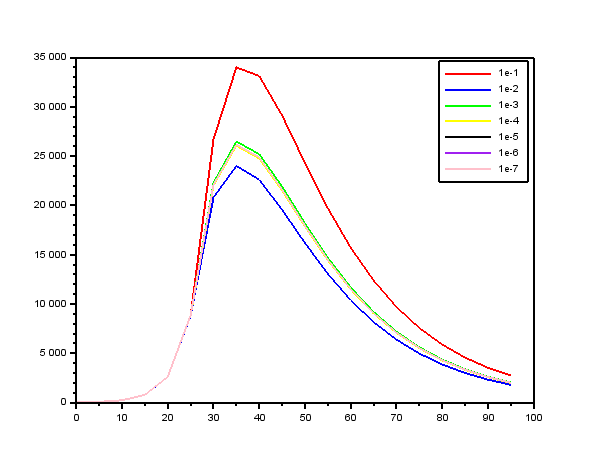
\includegraphics[width=0.7\linewidth]{./figures/tolerance_time_rkf_further_no_event_sci}
\caption{Time discontinuity model tolerance study on the Scilab version of RKF45 without discontinuity handling}
\label{fig:tolerance_time_rkf_further_no_event_sci}
\end{figure}

\begin{figure}[H]
\centering
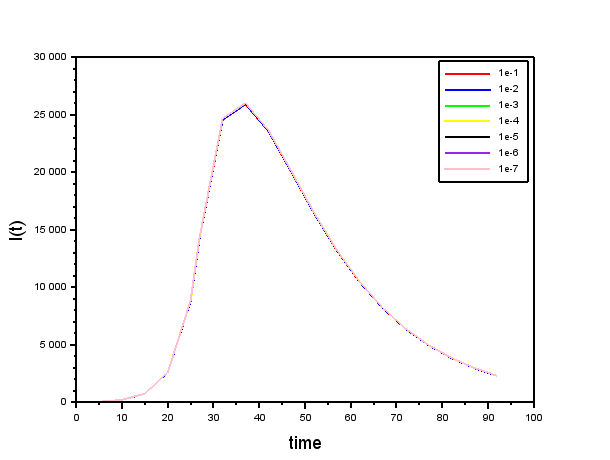
\includegraphics[width=0.7\linewidth]{./figures/tolerance_time_rkf_further_with_event_sci}
\caption{Time discontinuity model tolerance study on the Scilab version of RKF45 with discontinuity handling}
\label{fig:tolerance_time_rkf_further_with_event_sci}
\end{figure}

Figures $\ref{fig:tolerance_time_rkf_further_no_event_sci}$ and $\ref{fig:tolerance_time_rkf_further_with_event_sci}$ show a clear indication regarding why discontinuity handling is important. We can see that without it, we need a tolerance of $10^{-3}$ to get reasonably accurate results but with the discontinuity handling, we can use a tolerance of $10^{-1}$. We note that the use of such a coarse tolerance may mean that we still do not have the output points spaced out enough but the impact on the number of function evaluations, shown in Table $\ref{tab:tolerance_time_discontinuity_rk45_spaced_out_scilab}$, is clear.

\begin{table}[H]
\caption {Scilab RKF45 Spaced Out Time Discontinuity tolerance study} 
\label{tab:tolerance_time_discontinuity_rk45_spaced_out_scilab} 
\begin{center}
\begin{tabular}{ c c c }
tolerance & no discontinuity handling & with discontinuity handling\\ 
0.1 & 133 & 134 \\
0.01 & 166 & 152 \\
0.001 & 208 & 176 \\
1e-4 & 322 & 254 \\
1e-5 & 417 & 338 \\
1e-6 & 606 & 482 \\
1e-7 & 864 & 704 \\
\end{tabular}
\end{center}
\end{table}

Table $\ref{tab:tolerance_time_discontinuity_rk45_spaced_out_scilab}$ shows how the number of function evaluations with discontinuity handling is smaller. We also note that at coarse tolerance the number of function evaluations is similar but that at those tolerances, the code without discontinuity handling is not obtaining reasonably accurate results. We can thus conclude that using discontinuity handling lets us use coarser tolerances and leads to a smaller number of function evaluations while improving accuracy.


\subparagraph{Time discontinuity model tolerance study on the Matlab version of DOPRI5}
We perform the same experiment using $ode45$ in Matlab. We set both the absolute and relative tolerance to a particular tolerance and we see how the solvers perform. We remember that the default tolerance $ode45$ did not give a reasonably accurate solution. We note that it did not have a smaller default tolerance than $ode15s$. In this section, we show that with a sharper tolerance, $ode45$ is also capable of solving the problem without discontinuity handling but we will see that it is more efficient with discontinuity handling. Discontinuity handling will, again, allow us to use coarser tolerances.

\begin{figure}[H]
\centering
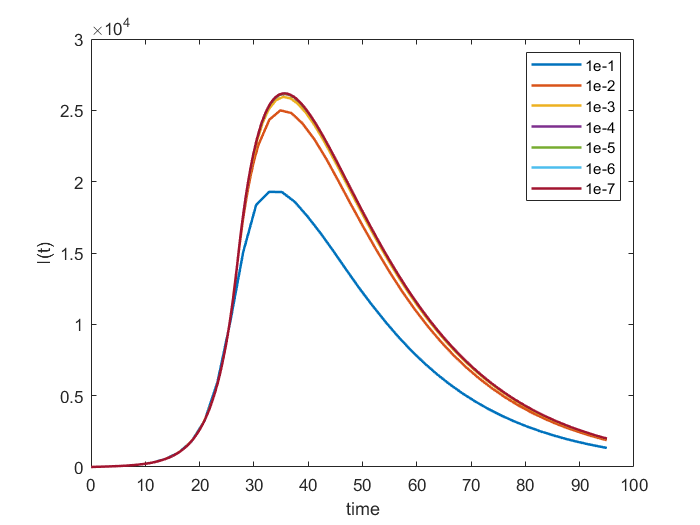
\includegraphics[width=0.7\linewidth]{./figures/tolerance_time_rk45_no_event_matlab}
\caption{Time discontinuity model tolerance study on the Matlab version of DOPRI5 without discontinuity handling}
\label{fig:tolerance_time_rk45_no_event_matlab}
\end{figure}

We first note from Figure $\ref{fig:tolerance_time_rk45_no_event_matlab}$ that at sufficiently sharp tolerances, we can get a reasonably accurate answer without discontinuity handling when the default tolerances did not give a reasonably accurate solution.

\begin{figure}[H]
\centering
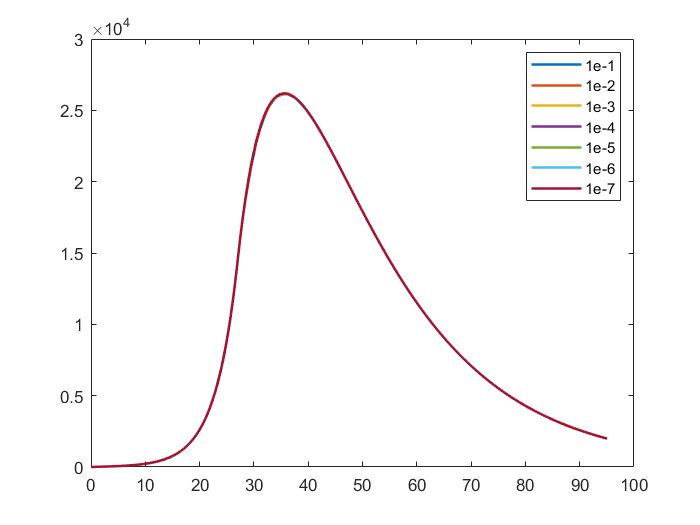
\includegraphics[width=0.7\linewidth]{./figures/tolerance_time_rk45_with_event_matlab}
\caption{Time discontinuity model tolerance study on the Matlab version of DOPRI5 with discontinuity handling}
\label{fig:tolerance_time_rk45_with_event_matlab}
\end{figure}

From Figures $\ref{fig:tolerance_time_rk45_no_event_matlab}$ and $\ref{fig:tolerance_time_rk45_with_event_matlab}$ we see that discontinuity handling allows us to use coarser tolerances while getting a reasonably accurate answer. We note that we could use a tolerance of $10^{-1}$ with discontinuity handling but we had to use a tolerance of $10^{-3}$ to get a reasonable solution. We will also see that discontinuity handling allows the solver to use fewer function evaluations in Table $\ref{tab:tolerance_time_discontinuity_rk45_matlab}$.

\begin{table}[H]
\caption {Matlab's DOPRI5 Time Discontinuity tolerance study} 
\label{tab:tolerance_time_discontinuity_rk45_matlab} 
\begin{center}
\begin{tabular}{ c c c }
tolerance & no discontinuity handling & with discontinuity handling\\ 
0.1 & 85 & 146 \\
0.01 & 121 & 146 \\
0.001 & 169 & 158 \\
0.0001 & 229 & 200 \\
1e-05 & 355 & 302 \\
1e-06 & 547 & 446 \\
1e-07 & 823 & 692 \\
\end{tabular}
\end{center}
\end{table}

Table $\ref{tab:tolerance_time_discontinuity_rk45_matlab}$ show that at coarser tolerances the solver without discontinuity handling use fewer function evaluations. However, at these tolerances, the solver did not give a reasonably accurate solution. At shaper tolerances, where the solver without discontinuity handling gives a reasonably accurate solution, the number of function evaluations for the solver with discontinuity handling is lower.


\section{State dependent discontinuity problem}
In this section, we consider the state-dependent discontinuity problem. We start by noting that this problem cannot be solved with the form of discontinuity handling used in the previous problem as we do not know when the discontinuity arises. Also, this problem will be harder than the time-dependent discontinuity problem as the parameter $\beta$ will be changed more than once as we attempt to model the waves of imposition of Covid-19 measures followed by periods where these measures are removed. 

As in Section $\ref{section:time_problem}$, changes in the modelling parameter $\beta$ introduce discontinuities in the function $f(t, y(t))$ and thus some solvers will ``thrash" when trying to solve the problem (as described in Section $\ref{subsection:effect_of_discontinuity}$). We will show that the presence of several discontinuities makes the problem hard enough that all the ODE solvers we considered, even at very sharp tolerances, will not be able to solve the problem with reasonable accuracy.

The problem uses the state variable, E, which is the number of Exposed people, to determine when to change the parameter $\beta$. When the number of exposed people is greater than 25000, measures will be introduced and thus $\beta$ will change from 0.9 to 0.005. When the number of exposed people drops to 10000, the measures will be relaxed and $\beta$ is set to 0.9. We run this model over a longer time period toggling the parameter $\beta$ back and forth to model the waves of alternating the imposition and relaxing of the measures. This scenario corresponds to the case of an unvaccinated population where the only means of controlling the spread of the virus is through measures such as social isolation, masking, etc... The ability of the virus to infect people is not diminished as time progresses, and when measures to stop the spread of the virus are removed, the infection rate of the virus returns to its original value.

We start with a naive treatment of the problem with if-statements applied inside the function that defines the right-hand side of the ODE system. We proceed to show how the problem cannot be solved this way even at sharp tolerances and finally, we will introduce a way to efficiently and accurately solve the problem using event detection.

\subsection{Naive treatment of Covid-19 state dependent discontinuity model}
\label{subsection:naive_state_problem}
The naive treatment of this problem is to use global variables for tracking when measures are implemented and relaxed and to toggle these global variables as we reach the required thresholds. Global variables are needed because we need to know if the number of Exposed people is going up or down to know whether we need to check for the maximum or the minimum threshold. We then have an if-statement that will choose the value of parameter $\beta$ based on whether measures are being implemented. The pseudo-code for this algorithm is as follows:

\begin{minipage}{\linewidth}
\begin{lstlisting}[language=Python]
measures_implemented = False
direction = "up"

function model_with_if(_, y):
    // ...
    global measures_implemented, direction
    if (direction == "up"):
        if (E > 25000):
            measures_implemented = True
            direction = "down"
    else:
        if (E < 10000):
            measures_implemented = False
            direction = "up"

    if measures_implemented:
        beta = 0.005 
    else:
        beta = 0.9
    // ...
    return (dSdt, dEdt, dIdt, dRdt)
\end{lstlisting}
\end{minipage}

\subsubsection{Solution to the state dependent discontinuity model in R}
\begin{figure}[H]
\centering
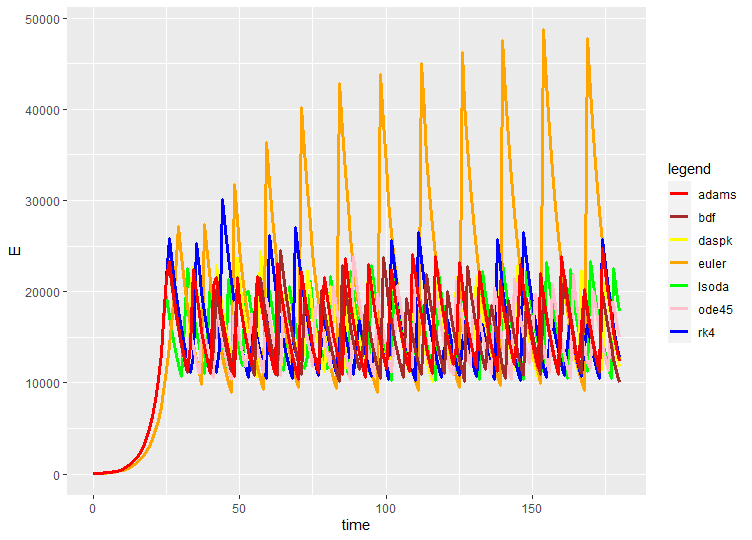
\includegraphics[width=0.7\linewidth]{./figures/state_discontinuity_R}
\caption{State dependent discontinuity model in R}
\label{fig:state_discontinuity_R}
\end{figure}
Figure $\ref{fig:state_discontinuity_R}$ shows how difficult this problem is with a naive treatment. We note that none of the solutions are aligned and that none of the solvers get the accurate solution (described in Section $\ref{subsection:state_with_event_detection}$) as none of the computed solutions cleanly oscillate between 10000 and 25000 with clear peaks and troughs.

We note that all the solvers, even the error-controlled ones, did not issue a warning about the integration and thus users may be tempted to think that their code has solved the problem to within reasonable accuracy. Having no warning also tells us that the error estimation and error control algorithms employed by all the solvers did not detect anything abnormal; the solvers return with an indication that the provided solutions are accurate to within the requested tolerance.

As we are modeling E, we expect that each graph should go from 25000 to 10000 and back to 25000 repeatedly but none of these graphs do so in the required pattern. We would also expect the solvers with error control to repeatedly reduce the step-size to satisfy the tolerance and compute solutions that align with each other but Figure $\ref{fig:state_discontinuity_R}$ shows that this is not the case.

We also note that the result for `euler' is especially poor as it reaches a maximum of 40000. This is again as expected as `euler' has no error control; `rk4', the other fixed step-size method, is also performing poorly as we see the solution it computes reach approximately 30000 in its third peak. This is happening even though the space between the output points is as small as it was when we were investigating the time-dependent discontinuity problem. Because of this, we will not run any spacing of output points experiments in this section. The step-size for these fixed-step solvers is not small enough and further step-size reductions are needed.
`
Another important fact to note is how poorly `Radau', as shown in Figure $\ref{fig:state_discontinuity_radau_R}$, is performing. This is not a problem in the R programming environment as similar results will be seen in Python in the next section and in the Fortran code in Section $\ref{section:fortran_inaccuracies}$. The solution grows exponentially even after the parameter $\beta$ should be switched to 0.005 which should begin a decay.

We perform an analysis with the Fortran code in $\ref{section:fortran_inaccuracies}$ to show that $\beta$ is indeed 0.005 while this exponential growth is happening. 

\begin{figure}[h]
\centering
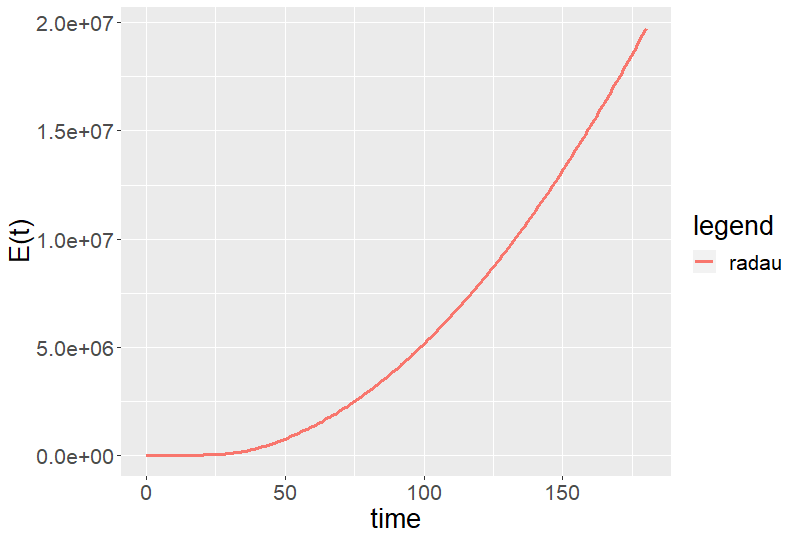
\includegraphics[width=0.7\linewidth]{./figures/state_discontinuity_radau_R}
\caption{State dependent discontinuity model of Radau in R}
\label{fig:state_discontinuity_radau_R}
\end{figure}

We then proceed to show that sharp tolerances are not enough to solve this problem as was the case for the time-dependent discontinuity problem. We repeated the experiment at the sharpest tolerance usable before some of the solvers failed. This was at $10^{-13}$ in the R environment. We set both the absolute and relative tolerance to that value and show the results in Figure $\ref{fig:state_discontinuity_sharp_R}$.

\begin{figure}[H]
\centering
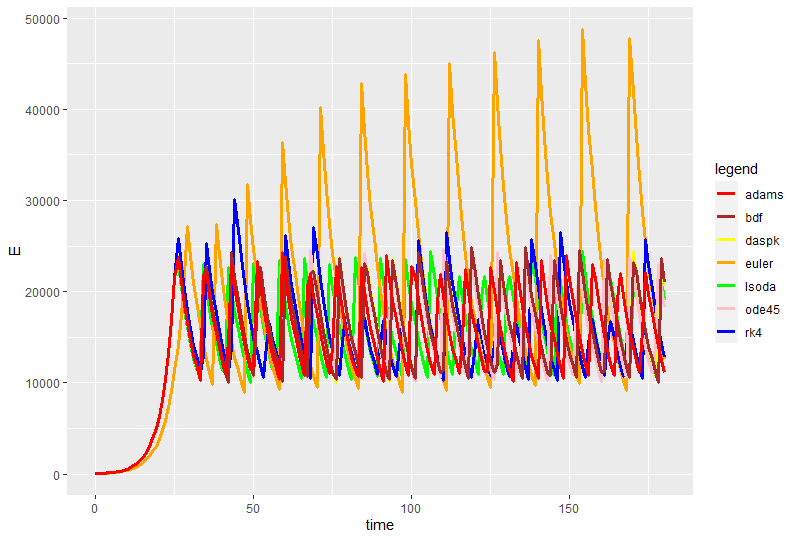
\includegraphics[width=0.7\linewidth]{./figures/state_discontinuity_sharp_R}
\caption{State dependent discontinuity model in R at high tolerances}
\label{fig:state_discontinuity_sharp_R}
\end{figure}

We can see from Figure $\ref{fig:state_discontinuity_sharp_R}$ that the situation has only marginally improved. None of the solvers give solutions that are in agreement and none of them cleanly oscillate between 10000 and 25000. We note that the error-controlled solvers are following the correct pattern and that until about time 20-30, some of them give solutions that are in agreement, showing that sharp tolerance error-control can step over one state-dependent discontinuity. (See the comparison against the final solution in Section $\ref{subsubsection:state_solution_comparison}$ to see that even this sharp tolerance solution is not accurate enough.)

The fixed step-size method `euler' and `rk4' are the same as in Figure $\ref{fig:state_discontinuity_R}$ since the codes do not employ a tolerance.

We can also point out that at such sharp tolerances, `Radau' longer computes solutions exhibiting the abnormal behavior we saw previously. From Figure $\ref{fig:state_discontinuity_radau_sharp_R}$, we can see that it oscillates approximately between 10000 and 25000. From supplementary experiments, we observe that `Radau' starts performing at a level that is comparable to the other solvers at a tolerance of $10^{-9}$.

\begin{figure}[H]
\centering
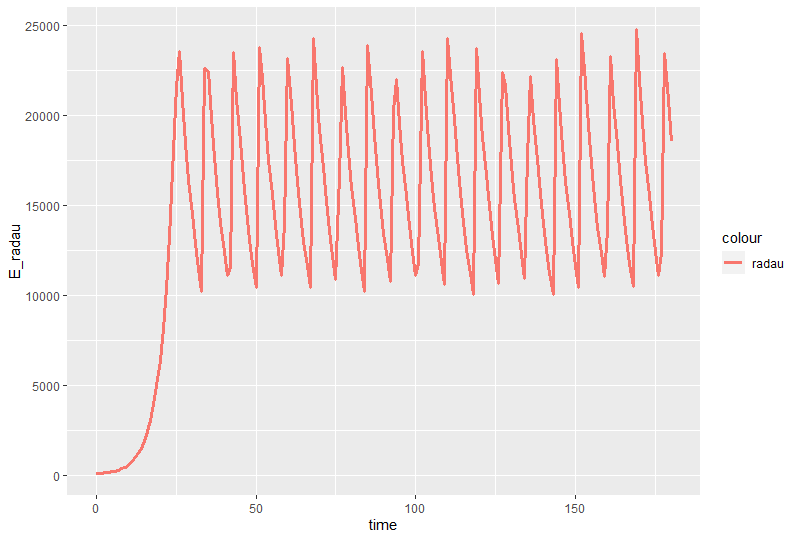
\includegraphics[width=0.7\linewidth]{./figures/state_discontinuity_sharp_radau_R}
\caption{State dependent discontinuity model of Radau in R at high tolerances}
\label{fig:state_discontinuity_radau_sharp_R}
\end{figure}

\subsubsection{Solution to the state dependent discontinuity model in Python}
\begin{figure}[H]
\centering
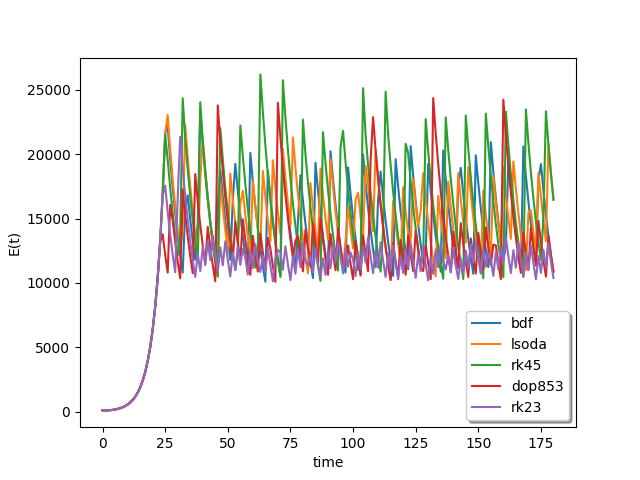
\includegraphics[width=0.7\linewidth]{./figures/state_discontinuity_py}
\caption{State dependent discontinuity model in Python}
\label{fig:state_discontinuity_python}
\end{figure}
Figure $\ref{fig:state_discontinuity_python}$ shows what happens when the problem is coded with global variables and if-statements in Python. We can see that the results are similar to those in R. This happens even though all solvers in Python have error control.

We note that all the solvers except `RK23' give solutions that at least oscillate between 10000 and 25000, though in completely dissimilar patterns. The solutions have peaks and troughs at different times and no warnings were given by the solvers.

The `RK23' solver, in purple, computes a solution with a completely different pattern than the other solvers. It never reaches 25000 and only oscillates between around 10000 and 15000. 

Again, as shown in Figure $\ref{fig:state_discontinuity_radau_py}$, `Radau' computes a solution that has E grow exponentially even though the parameter $\beta$ is eventually set to 0.005 which leads to a solution with an exponential decay in the E component with all other solvers.

\begin{figure}[h]
\centering
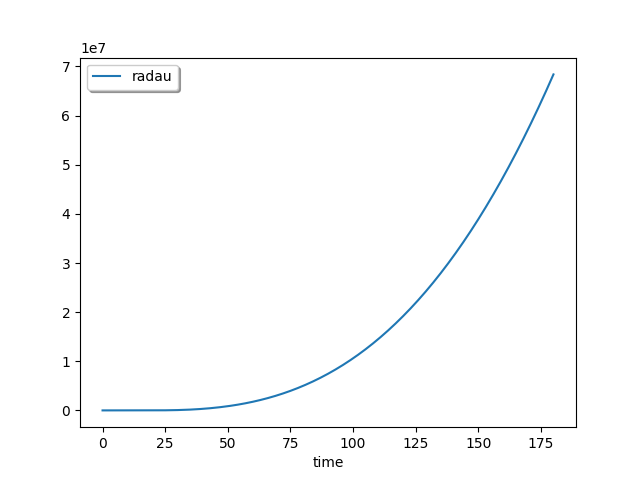
\includegraphics[width=0.7\linewidth]{./figures/state_discontinuity_radau_py}
\caption{State dependent discontinuity model of Radau in Python}
\label{fig:state_discontinuity_radau_py}
\end{figure}

We then used very sharp tolerances to solve the problem but, as is the case in the R environment, none of the solvers obtained a reasonably accurate solution. The highest tolerance we could use in Python without any one method failing was $10^{-12}$. Both the absolute and relative tolerances were set to this value and Figure $\ref{fig:state_discontinuity_sharp_python}$ shows the results from this sharp tolerance experiment.

\begin{figure}[H]
\centering
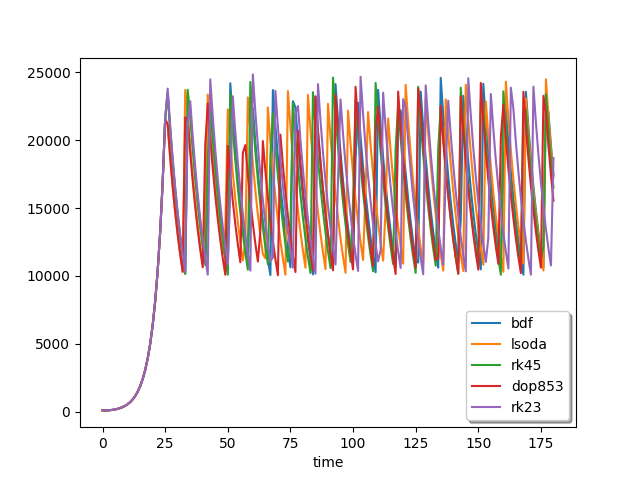
\includegraphics[width=0.7\linewidth]{./figures/state_discontinuity_sharp_py}
\caption{State dependent discontinuity model in Python at sharp tolerances}
\label{fig:state_discontinuity_sharp_python}
\end{figure}

Figure $\ref{fig:state_discontinuity_sharp_python}$ shows that the results did improve. However, the solvers give solutions that are not in agreement. We note that none of the solvers are oscillating beyond 25000 as was the case with the fixed-step solvers in R. At sharp tolerances, the solutions are aligned for the first few discontinuities with only some blurring until about t=25 when the solvers give substantially different solutions. Though the pattern is correct, none of the solvers give solutions that are in agreement telling us that none got the accurate solution that we present in Section $\ref{subsection:state_with_event_detection}$. (See the comparison against the final solution in Section $\ref{subsubsection:state_solution_comparison}$ to see that even this sharp tolerance solution is not accurate enough.)

We note that `RK23' is now following the correct pattern in that it oscillates between 10000 and 25000 whereas it only reached 15000 at the default tolerances. 

\begin{figure}[H]
\centering
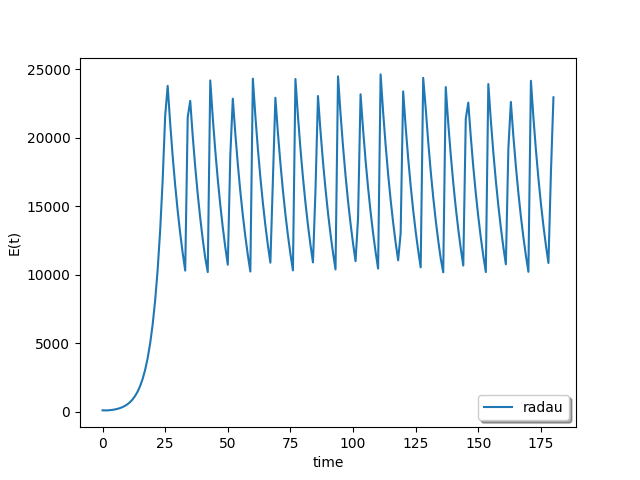
\includegraphics[width=0.7\linewidth]{./figures/state_discontinuity_sharp_radau_py}
\caption{State dependent discontinuity model of Radau in Python at sharp tolerances}
\label{fig:state_discontinuity_sharp_radau_py}
\end{figure}

Again, as shown in Figure $\ref{fig:state_discontinuity_sharp_radau_py}$, `Radau' begins to give reasonable solutions at these sharp tolerances; those solutions follows the pattern we are expecting but as we will show in Section $\ref{subsection:state_with_event_detection}$, they are still not sufficiently accurate solutions. `Radau' starts reasonably performing well at around a tolerance of $10^{-10}$. We also note that the R and Python implementation of `Radau' are different. The `Radau' solver in Python is implemented in Python with the NumPy library whereas R uses the Fortran code. Thus we eliminate the possibility of a bug in the code as well as any problem stemming from the interface from R to Fortran or from Python to NumPy. The problem is simply in how the Radau algorithm interacts with this naive implementation of the state-dependent discontinuity. In our experiments with the Radau Fortran code, in Section $\ref{section:fortran_inaccuracies}$, the same behavior is observed.

\subsubsection{Solution to the state dependent discontinuity model in Scilab}
\begin{figure}[H]
\centering
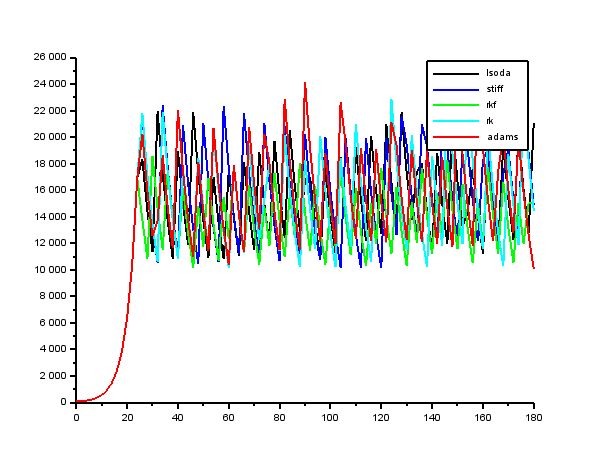
\includegraphics[width=0.7\linewidth]{./figures/state_discontinuity_scilab}
\caption{State dependent discontinuity model in Scilab}
\label{fig:state_discontinuity_scilab}
\end{figure}

Figure $\ref{fig:state_discontinuity_scilab}$ shows the same issues that we saw before. None of the solvers give solutions that are aligned which prompts us to conclude that none of them are getting an accurate solution. All of the solvers in Scilab have error control and we can also see that their solutions all follow the correct pattern of oscillating between 10000 and 25000. However, as we will discuss in Section $\ref{subsection:state_with_event_detection}$, none of the solutions are very accurate. We note that the spacing between output points is not important in this analysis as at the current spacing, even the solvers that depend on the spacing are getting inaccurate answers.

We then repeat the experiment at sharp tolerances. The Scilab rkf' method does not allow the use of very sharp tolerance as it has a cap of 3000 derivatives so it was omitted from this experiment. The sharpest tolerance we can use in Scilab before the other methods fail is $10^{-13}$; the results are shown in Figure $\ref{fig:state_discontinuity_sharp_scilab}$.

\begin{figure}[H]
\centering
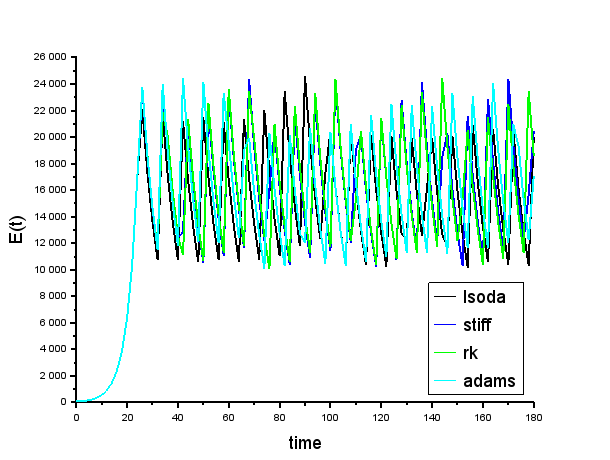
\includegraphics[width=0.7\linewidth]{./figures/state_discontinuity_sharp_sci}
\caption{State dependent discontinuity model in Scilab with sharp tolerances}
\label{fig:state_discontinuity_sharp_scilab}
\end{figure}

Again, in Figure $\ref{fig:state_discontinuity_sharp_scilab}$ we can see that the use of sharp tolerances is not enough to force the solvers to compute accurate solutions. The solutions did improve as all the solvers follow the correct pattern but none oscillate between 10000 and 25000 with clear peaks and troughs at those values. For the time period between 0 to 30, the solutions all seem to show reasonable agreement but as we go further in time, all of the solutions diverge. We also note that none of the solvers compute solutions in reasonable agreement with the solution discussed in Section $\ref{subsection:state_with_event_detection}$. (See the comparison against the final solution in Section $\ref{subsubsection:state_solution_comparison}$ to see that even these sharp tolerance solutions are not accurate enough.)


\subsubsection{Solution to the state dependent discontinuity model in Matlab}
\begin{figure}[H]
\centering
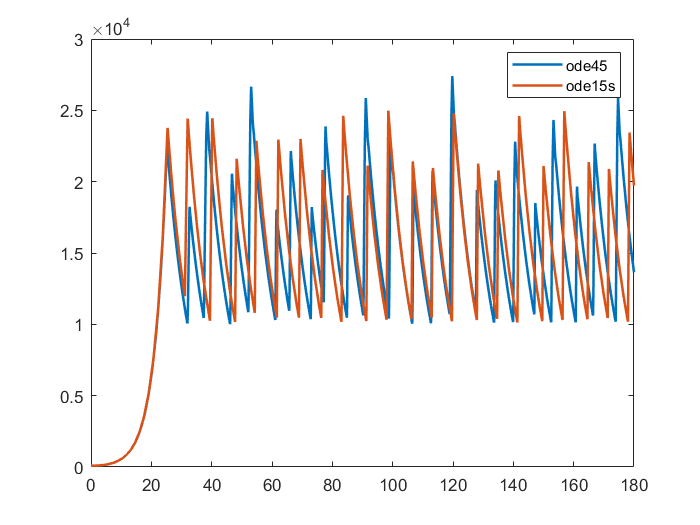
\includegraphics[width=0.7\linewidth]{./figures/state_discontinuity_matlab}
\caption{State dependent discontinuity model in Matlab}
\label{fig:state_discontinuity_matlab}
\end{figure}
We see the same incorrect solutions in Matlab at the default tolerances in Figure $\ref{fig:state_discontinuity_matlab}$. The solvers do not even consistently reach 25000. We then use a sharper tolerance to see how the solvers act.

\begin{figure}[h]
\centering
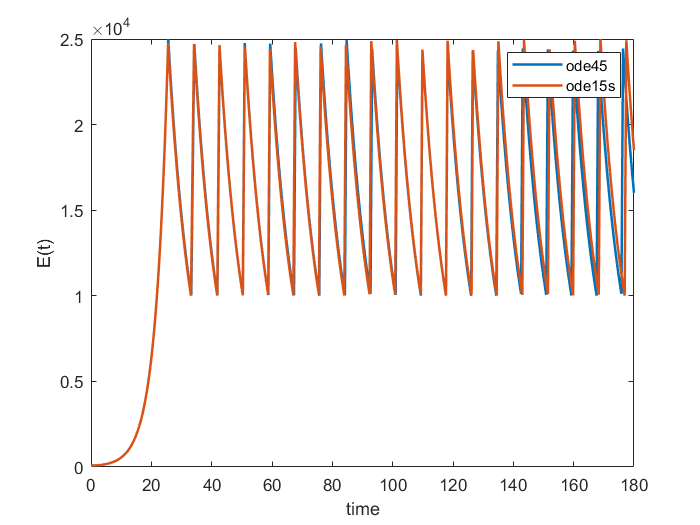
\includegraphics[width=0.7\linewidth]{./figures/state_discontinuity_sharp_matlab}
\caption{State dependent discontinuity model in Matlab with sharp tolerances}
\label{fig:state_discontinuity_sharp_matlab}
\end{figure}

Figure $\ref{fig:state_discontinuity_sharp_matlab}$ shows the results of the experiment at sharp tolerances. We get surprisingly good solutions compared to the solutions in the previous environments. However, as we will see in Section $\ref{subsection:state_with_event_detection}$, these solutions are computed extremely inefficiently and they are not as accurate as the solution presented in Section $\ref{subsection:state_with_event_detection}$, especially for later time periods. (See the comparison against the final solution in Section $\ref{subsubsection:state_solution_comparison}$ to see that even these sharp tolerance solutions are not accurate enough.)


\subsubsection{State dependent discontinuity model - solution comparison}
\label{subsubsection:state_solution_comparison}
In all the previous subsections, we have maintained that even the sharp tolerance solutions, though more in agreement, are not accurate. Here, we present a comparison between LSODA in Python at default tolerance, at the sharpest tolerance, and the final solution we will present shortly. We can see from Figure $\ref{fig:comparison_state_default_sharp_event}$ that the solution both at default and the sharp tolerance does not agree with the accurate solution. 

\begin{figure}[H]
\centering
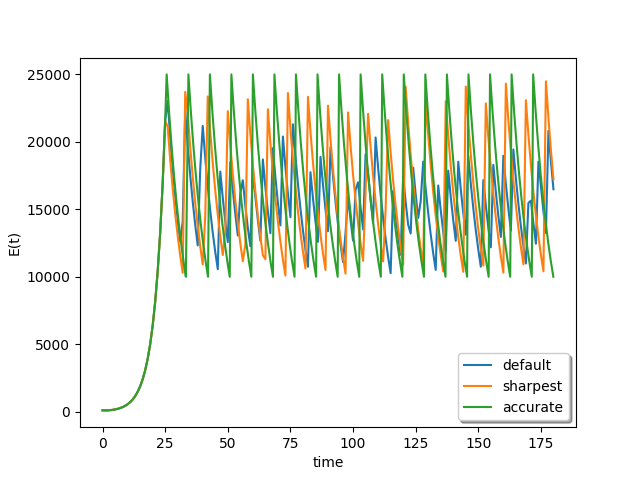
\includegraphics[width=0.7\linewidth]{./figures/comparison_state_default_sharp_event}
\caption{State dependent discontinuity model solutions comparison}
\label{fig:comparison_state_default_sharp_event}
\end{figure}

We also note that at the default tolerance, the solver uses 2357 function evaluations; at the sharpest tolerance, the solver uses 4282 evaluations; while for the solution obtained using event detection, the solver uses 535 function evaluations.

\subsection{Why the solvers fail even with sharp tolerances}
\label{subsection:state_sharp_tol_failed}
In this section we discuss why sharp tolerances were not enough to force the solvers to solve the problem in the naive way it is coded, i.e, using global variables and if-statements. 

Whenever there is a change in the value of $\beta$, the step that first encounters the ensuing discontinuity will almost always fail. As discussed in Section $\ref{subsection:effect_of_discontinuity}$, the step-size at a discontinuity will always have to be much smaller than the step-size on a continuous region. Thus the first encounter of a solver with any discontinuity will always be in the context of a failed step.

During this failed step, the value of the E will cross the threshold. The global variables will thus be toggled. But then, when the solver attempts to retake the step using a smaller step-size, to the left of the discontinuity, it will be using the wrong $\beta$ value. 

This observation is crucial as it allows us to conclude that just before the discontinuity, the function evaluations should be based on the previous $\beta$ value but they are in fact using the new $\beta$ value. There is no trivial way to code this behavior in the ODE function, $f(t, y(t))$, if we do not know the time of the discontinuity. 

The problem, in summary, is that the solvers need to figure out how to step up to the discontinuity such that to the left of the discontinuity, the step employs function evaluations that use the previous $\beta$, and then after the discontinuity, the solver employs function evaluations that use the new $\beta$ value. This cannot be coded in a straightforward way using the interfaces available in our programming environments.

At extremely sharp tolerances, the first step that encounters the discontinuity can also fail. The solver will still have to retake the step but, as discussed before, it will use the wrong $\beta$ value. In the next few sections, we will present the correct way to code problems with state-dependent discontinuities so that we get accurate solutions efficiently.

\subsection{Introducing event detection}
\label{subsection:intro_event_detection}
For the time-dependent discontinuity problem, we saw that if we used error-controlled software, then the solvers can work through one discontinuity at sufficiently high tolerances. We also showed that this was not the most efficient way for them to solve the problem. For the state-dependent discontinuity problem, we showed in the previous section why the solvers, using even sharp tolerances, will not be able to solve this problem with much accuracy. Because we do not know when the discontinuities occur, we cannot use the discontinuity handling technique, involving a cold restart, that we used to solve the time-dependent discontinuity problem. However, the idea that we developed in Section $\ref{subsection:time_disc_handling}$ about integrating continuous sub-problems separately and combining them into a final solution can still be applied here. 

To integrate continuous sub-problems, we need a way to detect that a threshold has been met, and then as soon as we reach such a point, we can perform a cold start. This will make the solver integrate the problem one continuous subinterval at a time. In this section, we will explain the capability of modern solvers to detect events and we will show how to encode the E(t) thresholds (either E(t)=25000 or E(t)=10000) as events so that the times at which they occur can be determined. We can then perform a cold start at these times.

To perform event detection, an ODE solver will require two functions from the user: the usual ODE right-hand side function, $f(t, y(t))$ and another function which we will call the root function (commonly denoted by $g(t, y(t))$), that determines the events.

The root function is a function that, given the value of the solution to the ODE at the current step will return a real number. The ODE solution is said to have a root whenever the value of the root function is zero. The key idea is that each event must be written so that it occurs at the root of a root function.

The solver calls the root function at the end of each successful step that it takes and will record its value. It will then compare the value of the root function with the corresponding value from the previous step to see if there has been a change of sign. If the value of the root-function has changed sign, the solver raises a flag to say that it has detected a root and will then run a root-finding algorithm on that step to find the point where the root-function equals zero. Most solvers will then return, allowing us to perform a cold start.

Using event detection thus entails defining a function that takes the value of the ODE solution at the current point and returns a real number which is zero whenever we want it to detect an event. For example, if we want to detect when x is 100, it is sufficient to define (x - 100) to be the root function. In the next section, we will elaborate on how to use event detection to accurately and efficiently solve the state-dependent discontinuity problem.

We also mention that many modern solvers have event detection built-in. Thus users should be able to use event-detection solvers from their preferred programming environments without any additional software.

\subsection{Solving the state dependent discontinuity model using event detection}
\label{subsection:state_with_event_detection}
As mentioned earlier, each toggling between the values of the parameter $\beta$ introduces a discontinuity. As none of the provided solvers are designed to solve discontinuous problems, we get the erroneous solutions reported in $\ref{subsection:naive_state_problem}$. We have seen that although sharp tolerances do result in somewhat better solutions being computed, none of the solvers were able to obtain an accurate solution. The use of such sharp tolerances leads to inefficiencies as well. We will now present an approach using event detection that is both accurate and efficient.

The solution is to use the thresholds that we have defined in our model to define events and integrate up to each threshold using the event detection capability of the solver. We can then cold start from there and repeat the process with another right-hand side function corresponding to the new $\beta$ value and with a different root function that encodes the next threshold we are looking for. We repeat this process until we reach the end of the time interval. This approach allows the solvers to integrate continuous sub-problems, one at a time, and these sub-problems can then be combined into a final solution.

For our specific problem, event detection is used as follows:
We start by solving the problem with $\beta$=0.9 and with a root function that detects when E is equal to 25000. Once we detect the time at which E(t)=25000, we do a cold start. We extract the solution of the solver at the time of the event and use that solution as the initial value for our next call to the solver. This next call will have $\beta$ at 0.005 and a root function that detects a root when E(t)=10000. We again integrate up to that new threshold and cold start when we reach it. The new cold start will have $\beta$=0.9 and the root function looking for E(t)=25000 as the event. This is repeated until we reach the desired end time. The pseudo-code is as follows:

\begin{minipage}{\linewidth}
\centering
\begin{lstlisting}[language=Python]
function model_no_measures(t, y):
    beta = 0.9
    // code to get dSdt, dEdt, dIdt, dRdt
    return (dSdt, dEdt, dIdt, dRdt)

function root_25000(t, y):
    E = y[1]
    return E - 25000

function model_with_measures(t, y):
    beta = 0.005
    // code to get dSdt, dEdt, dIdt, dRdt
    return (dSdt, dEdt, dIdt, dRdt)

function root_10000(t, y):
    E = y[1]
    return E - 10000

res = array()
t_initial = 0
y_initial = (S0, E0, I0, R0)
while t_initial < 180:
    tspan = [t_initial, 180]
    if (measures_implemented):
        sol = ode(model_with_measures, tspan, y_initial,
            events=root_10000)
        measures_implemented = False
    else:
        sol = ode(model_no_measures, tspan, y_initial,
            events=root_25000)
        measures_implemented = True
    t_initial = extract_last_t_from_sol(sol)
    y_initial = extract_last_row_from_sol(sol)
    res = concatenate(res, sol)

// use res as the final solution
\end{lstlisting}
\end{minipage}

Some programming environments, such as Python, by default, do not stop the integration when the first event is detected. To do a cold start, we need the solver to stop at events, and to make this happen, in some programming environments we need to set appropriate flags. 

\subsubsection{Solving the state-dependent discontinuity model in R using event detection}
\begin{figure}[H]
\centering
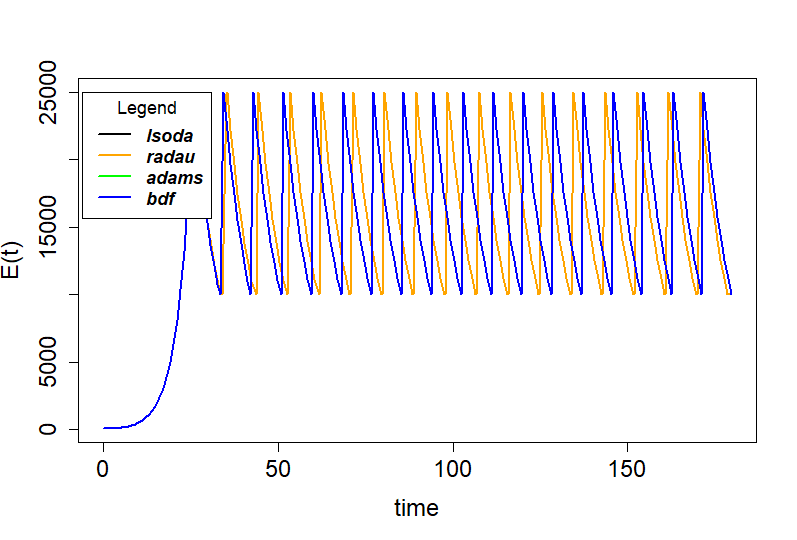
\includegraphics[width=0.7\linewidth]{./figures/solve_state_discontinuity_R}
\caption{Solving state discontinuity model in R}
\label{fig:solve_state_discontinuity_R}
\end{figure}
Several of the solvers in R have event detection capabilities. These are: `adams', `bdf', `lsoda', `Radau', and they will be used in this section to solve the model using the approach described in the previous subsection. From Figure $\ref{fig:solve_state_discontinuity_R}$, we can see that all the solvers give solutions that are in agreement except `Radau'. This is in contrast with what happened previously when we were integrating a discontinuous problem, even at sharp tolerances. 

The case of `Radau' is interesting as it was giving a poor quality solution at the default tolerances, without event detection but it is now giving at least a solution that is exhibiting a correct pattern. We note that at high tolerances `Radau' with event detection approach the results from the other solvers, as shown in Figure $\ref{fig:solve_state_discontinuity_sharp_R}$. We will also note the poor performance of Radau in Table $\ref{tab:state_discontinuity_R}$. We also note that `Radau' Fortran code does not have built-in detection and that the event detection has been added through the C interface, which may explain the slight disparity.

\begin{figure}[H]
\centering
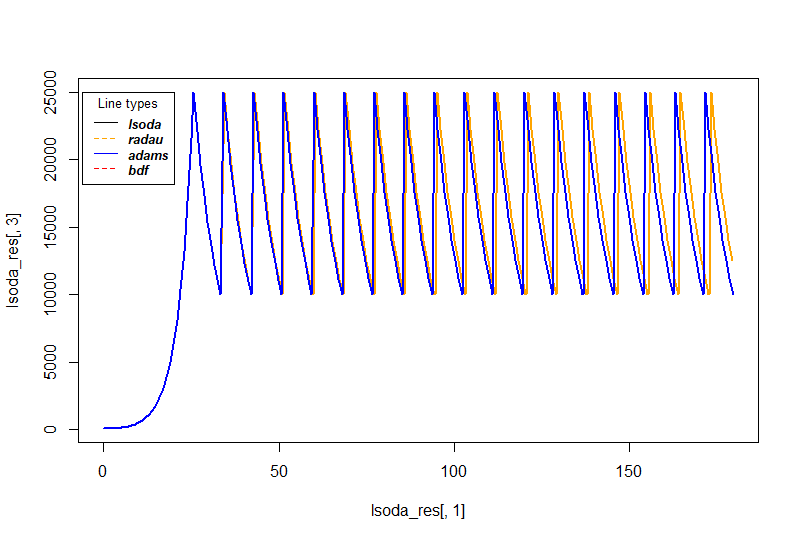
\includegraphics[width=0.7\linewidth]{./figures/solve_state_discontinuity_sharp_R}
\caption{Solving state discontinuity model at sharp tolerances in R}
\label{fig:solve_state_discontinuity_sharp_R}
\end{figure}

We will show in Table $\ref{tab:state_discontinuity_R}$ that introducing event detection also made the solvers significantly more efficient while giving us better results.

We note that it is unfair to compare the efficiency of the solvers at the default tolerances with the efficiency of the solvers when they use event detection as the results for the former are inaccurate.

\begin{table}[h]
\caption {R state discontinuity model} 
\label{tab:state_discontinuity_R}
\begin{center}
\begin{tabular}{ c c c c c } 
method & no event & no event-sharp tol. & with event & with event-sharp tol.\\ 
lsoda & 2135 & 4658 & 1248 & 3435 \\
radau & 1002 & 21835 & 2151 & 14681\\
bdf & 3300 & 9803 & 1678 & 7963\\
adams & 1368 & 3467 & 817 & 2689\\
\end{tabular}
\end{center}
\end{table}

We can see from Table $\ref{tab:state_discontinuity_R}$ that with event detection we are gaining an improvement of around 1000 function evaluations for `lsoda', 7000 in `Radau' (sharp tol comparison), 2000 in `bdf', and 500 in `adams' while having more accuracy. This significant decrease in the number of function evaluations will lead to much faster CPU times, especially when the right-hand side function, $f(t, y)$ is more complex.

Also, we can see from the table that the solvers use fewer function evaluations compared with event detection than without event detection at the default tolerances. When comparing the values at the sharp tolerances, the use of event detection also decreased the respective number of function evaluations.

We also note that the Fortran code for `Radau' does not have event detection and that event detection was added through the R interface.

\subsubsection{Solving the state-dependent discontinuity model in Python using event detection}
\begin{figure}[H]
\centering
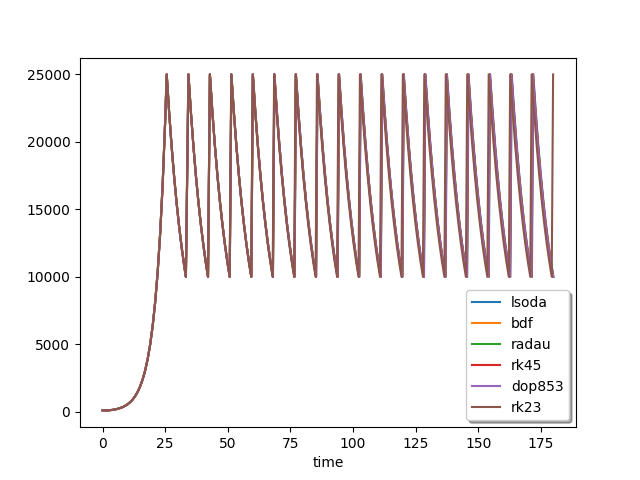
\includegraphics[width=0.7\linewidth]{./figures/solve_state_discontinuity_py}
\caption{Solving state dependent discontinuity model in Python}
\label{fig:solve_state_discontinuity_py}
\end{figure}
All the solvers in Python have event detection and thus all will be used in this part of the study. In Python, $solve\_ivp()$ does not stop when an event is detected by default. We thus need to set the terminal flag of the root functions.
(Example: $root\_10000.terminal = True$).
Again, Figure $\ref{fig:solve_state_discontinuity_py}$ shows that all the solvers give solutions that are in agreement, suggesting that this is the correct solution. This is different from our results at sharp tolerances when event detection was not employed. We will also see that this is a much more efficient approach across all the solvers. The $solve\_ivp()$ implementation of `Radau' is in Python itself and thus it is different from the R implementation. We note that we did not have to provide it with a sharp tolerance to make it align with the other solvers, suggesting that the issue in R may be due to the C implementation of event detection.

As is the case with R, we cannot compare the default tolerance efficiency data to the event detection efficiency data as the former corresponds to inaccurate results. So, in Table $\ref{tab:state_discontinuity_Py}$, we compare the sharp tolerance efficiency data with the data from the event detection computation.

\begin{table}[h]
\caption {Python state discontinuity model} \label{tab:state_discontinuity_Py}
\begin{center}
\begin{tabular}{ c c c c } 
method & no event & no event with sharp tol. & with event detection \\ 
lsoda & 2357 & 4282 & 535 \\
bdf & 2301 & 11794 & 808 \\
radau & 211 & 74723 & 990 \\
rk45 & 1484 & 17648 & 674 \\
dop853 & 11129 & 21131 & 1514 \\
rk23 & 4307 & 246644 & 589 \\
\end{tabular}
\end{center}
\end{table}

Table $\ref{tab:state_discontinuity_Py}$ shows that the number of function evaluations when the solvers use event detection is far less when they do not; `LSODA' used around 3000 fewer function evaluations, `BDF' used 11000 less, `Radau' used 74000 less, `RK45' used 17000 less, `DOP853' used 20000 less and `RK23' used 246000 less. The reduction in CPU times from this will be significant across all the solvers, especially with a more complex right-hand side function.

\subsubsection{Solving the state-dependent discontinuity model in Scilab using event detection}
\begin{figure}[H]
\centering
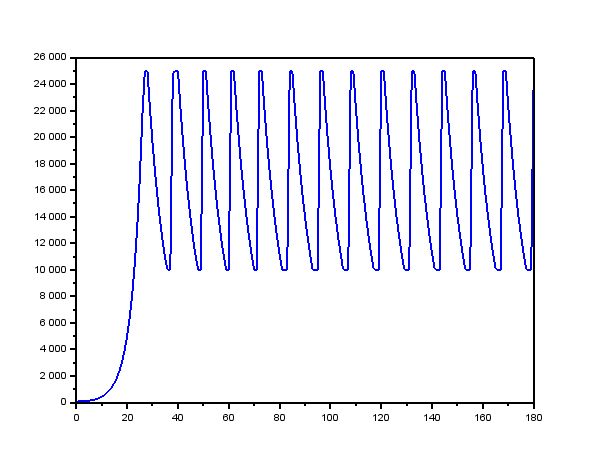
\includegraphics[width=0.7\linewidth]{./figures/solve_state_discontinuity_scilab}
\caption{Solving state discontinuity model in Scilab}
\label{fig:solve_state_discontinuity_scilab}
\end{figure}
There is only one solver with root functionality in Scilab; it is `lsodar', the root-finding version of `lsoda'. Judging from the solutions we obtained from Python and R, it seems that `lsodar' gave a correct solution as well. It oscillates in the correct pattern and goes sharply between 10000 and 25000.

\begin{table}[h]
\caption {Scilab state discontinuity model} \label{tab:state_discontinuity_scilab}
\begin{center}
\begin{tabular}{ c c c c } 
method & no event & no event with sharp tol. & with event detection \\ 
lsoda & 2794 & 4636 & 1327 \\
\end{tabular}
\end{center}
\end{table}

From Table $\ref{tab:state_discontinuity_scilab}$, we can see that the root-finding code uses fewer function evaluations that `lsoda' both at sharp and default tolerances.

\subsubsection{Solving the state-dependent discontinuity model in Matlab using event detection}
\begin{figure}[H]
\centering
\includegraphics[width=0.7\linewidth]{./figures/solve_state_discontinuity_matlab}
\caption{Solving state discontinuity model in Matlab}
\label{fig:solve_state_discontinuity_matlab}
\end{figure}
Both $ode45()$ and $ode15s()$ have an event detection capability. (The root functions need to set that the root is terminal to perform a cold start.) We applied event detection to solve the problem with the solvers in the Matlab environment and the results are shown in Figure $\ref{fig:solve_state_discontinuity_matlab}$. We remember that the solutions in Matlab without event detection were surprisingly accurate but were in disagreement with each other at points further in time. We can see that with event detection, the solutions are all in agreement at the default tolerances even at points further in time. We also see, in Table $\ref{tab:state_discontinuity_matlab}$, that the use of event detection is also more efficient than the computation without event detection.

\begin{table}[h]
\caption {Matlab state discontinuity model problem} \label{tab:state_discontinuity_matlab}
\begin{center}
\begin{tabular}{ c c c c } 
method & no event & no event with sharp tol. & with event detection \\ 
ode45 & 2023 & 22411 & 859 \\
ode15s & 1397 & 11550 & 620 \\
\end{tabular}
\end{center}
\end{table}

We can see in Table $\ref{tab:state_discontinuity_matlab}$ that the computation with event detection uses fewer function evaluations than the code without event detection at default and sharp tolerances. We see that the computations with sharp tolerances, although they give acceptable solutions, use 20000 more function evaluations in $ode45$ than the computation with event detection and 11000 in the case of $ode15s$ than the computation with event detection.

\subsection{Efficiency data and tolerance study for the state dependent discontinuity problem}
\label{subsection:state_tolerance_study}
In this section, we will investigate how sharpening the tolerance improves the results in the case of the non-event detection experiment. We will also investigate coarsening the tolerance with event detection to show how coarse a tolerance we can use while getting acceptable results.

We will perform this analysis on LSODA across R, Python, and Scilab, as they appear to use the same source code, and with R and Python versions of DOPRI5 which do not use the same code but do use the same Runge-Kutta pair and with the Scilab version of RKF45 which is not the same code, nor the same pair but is a Runge-Kutta pair of the same order. We also use $ode45$ in Matlab as it is an implementation of DOPRI5 in Matlab. 

\subsubsection{Comparing LSODA across platforms for the state discontinuous problem}
\subparagraph{State dependent discontinuity LSODA tolerance study in R}
In this section, we use the R version of LSODA at multiple tolerances. We set both the relative and the absolute tolerance to various values and analyze the solution.

We know that without event detection, LSODA does not give accurate results even at very sharp tolerances. We will also examine how coarse we can set the tolerance to still have the event detection computation yield accurate results.

\begin{figure}[h]
\centering
\includegraphics[width=0.7\linewidth]{./figures/tolerance_state_lsoda_no_event_R}
\caption{State dependent discontinuity model tolerance study on the R version of LSODA without event detection}
\label{fig:tolerance_state_lsoda_no_event_R}
\end{figure}

\begin{figure}[h]
\centering
\includegraphics[width=0.7\linewidth]{./figures/tolerance_state_lsoda_with_event_R}
\caption{State dependent discontinuity model tolerance study on the R version of LSODA with event detection}
\label{fig:tolerance_state_lsoda_with_event_R}
\end{figure}

Figure $\ref{fig:tolerance_state_lsoda_no_event_R}$ shows that LSODA applied to the same problem at different tolerances gives vastly different results. We would expect the solutions at the sharper tolerances to be along very similar curves but that is not the case. The computation is suffering from the fact that the first step that encounters a discontinuity fails and switches the global variables. This further supports our statement that for any state-dependent discontinuity, we cannot get reasonable results simply by sharpening the tolerance.

From Figures $\ref{fig:tolerance_state_lsoda_with_event_R}$ and $\ref{fig:tolerance_state_lsoda_no_event_R}$, we can see the clear advantage of using event detection. Event detection even allows us to use very coarse tolerances while solving the problem to a reasonable accuracy. Event detection allows us to use tolerances of $10^{-3}$ and sharper to get reasonable results while the computation without event detection failed even at a tolerance of $10^{-13}$. We also analyze the differences in efficiency between the two codes in Table $\ref{tab:tolerance_state_discontinuity_lsoda_R}$.

\begin{table}[h]
\caption {R version of LSODA applied to state discontinuity model tolerance study} \label{tab:tolerance_state_discontinuity_lsoda_R} 
\begin{center}
\begin{tabular}{ c c c }
tolerance & no event detection & with event detection \\
1e-01 & 675 & 560 \\
1e-02 & 1856 & 522 \\
1e-04 & 1863 & 752 \\
1e-06 & 2135 & 1248 \\
1e-07 & 2676 & 1874 \\
1e-08 & 2730 & 2060 \\
1e-10 & 3337 & 2604 \\
1e-11 & 3603 & 3054 \\
\end{tabular}
\end{center}
\end{table}

Table $\ref{tab:tolerance_state_discontinuity_lsoda_R}$ shows a decrease in the number of function evaluations across all tolerances which will translate into faster CPU times when the right-hand side function is more complex. We note that the comparison is unfair as the computations without event detection do not give a reasonably accurate answer. Furthermore, the latter computation uses more function evaluations. This supports our conclusion that event detection is the appropriate way to solve state-dependent discontinuity problems when the discontinuity can be characterized in terms of an event.

\subparagraph{State dependent discontinuity model LSODA tolerance study in Python}
In this section, we use the Python version of LSODA at multiple tolerances to see how it performs. We note that LSODA without event detection even at very sharp tolerances in Python was still not giving accurate results but we will see how the solutions change as the tolerance is increased. We will also show that coarse tolerances can be used with the computation that uses event detection. 

\begin{figure}[h]
\centering
\includegraphics[width=0.7\linewidth]{./figures/tolerance_state_lsoda_no_event_py}
\caption{State dependent discontinuity model tolerance study on the Python version of LSODA without event detection}
\label{fig:tolerance_state_lsoda_no_event_py}
\end{figure}

\begin{figure}[h]
\centering
\includegraphics[width=0.7\linewidth]{./figures/tolerance_state_lsoda_with_event_py}
\caption{State dependent discontinuity model tolerance study on the Python version of LSODA with event detection}
\label{fig:tolerance_state_lsoda_with_event_py}
\end{figure}

Again Figure $\ref{fig:tolerance_state_lsoda_no_event_py}$ exposes that LSODA applied to the same problem at different tolerances give substantially different results. We would expect the computations at the sharper tolerances to give quite similar results but this is not the case.

From Figures $\ref{fig:tolerance_state_lsoda_with_event_py}$ and $\ref{fig:tolerance_state_lsoda_no_event_py}$, we can see that the addition of event detection allows for the use of a coarser tolerance. We also note that the computations with event detection blur as we go further in time. This is because the coarser tolerance computations are not giving a sufficiently accurate solution. In Python, it is at a tolerance of $10^{-4}$ and sharper that we get reasonably accurate results. 

We analyse the efficiency of the computations in Table $\ref{tab:tolerance_state_discontinuity_lsoda_py}$. We must note that this analysis is unfair as the computation without event detection does not give an accurate solution to the problem. Still, we will see that the event detection computation uses fewer function evaluations while getting a more accurate answer.

\begin{table}[h]
\caption {Python version of LSODA applied to state discontinuity model tolerance study} \label{tab:tolerance_state_discontinuity_lsoda_py} 
\begin{center}
\begin{tabular}{ c c c }
tolerance & no event detection & with event detection \\
0.1 & 1207 & 425 \\
0.01 & 1627 & 454 \\
0.0001 & 1968 & 689 \\
1e-06 & 2122 & 1305 \\
1e-07 & 2684 & 1807 \\
1e-08 & 2730 & 2099 \\
1e-10 & 3337 & 2639 \\
1e-11 & 3603 & 3098 \\
\end{tabular}
\end{center}
\end{table}

\subparagraph{State dependent discontinuity model LSODA tolerance study in Scilab}

We perform the same experiment in Scilab. We set the absolute and relative tolerance to the same values as in the other experiments and run the solvers. For the different tolerance values, we plot the solutions and analyze how the solutions computed without event detection change as the tolerance is sharpened; we also examine how coarse a tolerance we can use with the event detection solver.

\begin{figure}[h]
\centering
\includegraphics[width=0.7\linewidth]{./figures/tolerance_state_lsoda_no_event_sci}
\caption{State dependent discontinuity model tolerance study on the Scilab version of LSODA without event detection}
\label{fig:tolerance_state_lsoda_no_event_sci}
\end{figure}

\begin{figure}[h]
\centering
\includegraphics[width=0.7\linewidth]{./figures/tolerance_state_lsoda_with_event_sci}
\caption{State dependent discontinuity model tolerance study on the Scilab version of LSODA with event detection}
\label{fig:tolerance_state_lsoda_with_event_sci}
\end{figure}

Again, Figure $\ref{fig:tolerance_state_lsoda_no_event_sci}$ exposes the behavior whereby the same solver applied to the same problem at different tolerances gives substantially different results. We would expect the code at the sharper tolerances to give very similar curves but clearly, LSODA even at sharp tolerances does not.

From Figure $\ref{fig:tolerance_state_lsoda_with_event_sci}$, we can see that the use of the event detection allows us to use a smaller tolerance. We can use a tolerance of $10^{-3}$ and still get an accurate answer whereas, without event detection, even tolerance of $10^{-12}$ is not sufficient.

\begin{table}[h]
\caption {Scilab version of LSODA applied to state discontinuity model tolerance study} \label{tab:tolerance_state_discontinuity_lsoda_scilab} 
\begin{center}
\begin{tabular}{ c c c }
tolerance & no event detection & with event detection \\
0.1 & 1141 & 287 \\
0.01 & 1606 & 262 \\
0.0001 & 1968 & 523 \\
0.000001 & 2122 & 983 \\
0.0000001 & 2684 & 1307 \\
1.000D-08 & 2730 & 1567 \\
1.000D-10 & 3380 & 1963 \\
1.000D-11 & 3603 & 2331 \\
\end{tabular}
\end{center}
\end{table}

\subsubsection{Comparing Runge-Kutta pairs across platforms for state discontinuous problem}
In this section, we consider solvers based on Runge-Kutta pairs of the same order: DOPRI5 in R aliased as `ode45', DOPRI5 in Python aliased as `RK45', DOPRI5 in Matlab through the $ode45$ function, and RKF45 in Scilab aliased as `rkf'.

We recall that without event detection, none of these solvers across the platforms solved the problem correctly even with sharp tolerances. We will show what happens to these solvers as the tolerance is sharpened. We also coarsen the tolerance for the case where solvers use event detection where that is possible to see how coarse the tolerance can be while still obtaining sufficient accuracy.

\subparagraph{Tolerance study on state discontinuity using the R version of DOPRI5}
The R version of DOPRI5 does not have event detection but we still perform the experiment on this solver without event detection. We pick several values for the absolute and relative tolerances and run the solvers. In so doing we see how the code performs as the tolerance is sharpened. 

\begin{figure}[h]
\centering
\includegraphics[width=0.7\linewidth]{./figures/tolerance_state_rk45_no_event_R}
\caption{State dependent discontinuity model tolerance study on the R version DOPRI5 without event detection}
\label{fig:tolerance_state_rk45_no_event_R}
\end{figure}

From Figure $\ref{fig:tolerance_state_rk45_no_event_R}$, we see that DOPRI5 applied to the same problem with different tolerances, gives significantly different solutions.

We then report on the efficiency data for this case in Table $\ref{tab:tolerance_state_discontinuity_rk45_R}$. 

\begin{table}[h]
\caption {R version of DOPRI5 state discontinuity model tolerance study} \label{tab:tolerance_state_discontinuity_rk45_R} 
\begin{center}
\begin{tabular}{ c c }
tolerance & no event detection \\
1e-01 & 1082 \\
1e-02 & 1142 \\
1e-04 & 2014 \\
1e-06 & 2027 \\
1e-07 & 2193 \\
1e-08 & 2919 \\
1e-10 & 5194 \\
1e-11 & 7690 \\
\end{tabular}
\end{center}
\end{table}

\subparagraph{Tolerance study on state discontinuity using the Python version of DOPRI5}
We perform the same experiment in Python. The absolute and relative tolerances are set to a range of values and the solver is run both with and without event detection. We report on how the code performs as the tolerance is increased in the case without event detection. Since the Python version of DOPRI5 has event detection, we will see how coarse the tolerance can be set while still giving us a reasonably accurate solution. We note that the solver crashes if we ask for a tolerance of 0.1.

\begin{figure}[h]
\centering
\includegraphics[width=0.7\linewidth]{./figures/tolerance_state_rk45_no_event_py}
\caption{State dependent discontinuity model tolerance study on the Python version of DOPRI5 without event detection}
\label{fig:tolerance_state_rk45_no_event_py}
\end{figure}

\begin{figure}[h]
\centering
\includegraphics[width=0.7\linewidth]{./figures/tolerance_state_rk45_with_event_py}
\caption{State dependent discontinuity model tolerance study on the Python version of DOPRI5 with event detection}
\label{fig:tolerance_state_rk45_with_event_py}
\end{figure}

In Figure $\ref{fig:tolerance_state_rk45_no_event_py}$, we can see that even at sharp tolerances, the solver is not able to compute a reasonably accurate solution.

In contrast, when using event detection, the code can use very coarse tolerances. We can see that a tolerance of $10^{-4}$ is sharp enough to solve the given problem accurately; the blurring that occurs is due to the coarser tolerances. We present the efficiency data in Table $\ref{tab:tolerance_state_discontinuity_rk45_py}$ to show how the code with event detection is also far more efficient.

\begin{table}[h]
\caption {The Python version of DOPRI5 state discontinuity model tolerance study} \label{tab:tolerance_state_discontinuity_rk45_py} 
\begin{center}
\begin{tabular}{ c c c }
tolerance & no event detection & with event detection \\
0.01 & 1400.0 & 664.0 \\
0.0001 & 8462.0 & 806.0 \\
1e-06 & 6248.0 & 1232.0 \\
1e-07 & 6848.0 & 1754.0 \\
1e-08 & 7082.0 & 2354.0 \\
1e-10 & 10262.0 & 5066.0 \\
1e-11 & 13058.0 & 7688.0 \\
\end{tabular}
\end{center}
\end{table}

We can see in Table $\ref{tab:tolerance_state_discontinuity_rk45_py}$ that across all the different tolerances, the solver with event detection requires fewer function evaluations, around several thousand fewer for the sharper tolerances. 

\subparagraph{State dependent discontinuity RKF45 tolerance study in Scilab}
Scilab uses RKF45 which is a different Runge-Kutta pair from what is used in DOPRI5 but the pairs have the same order. It does not have event detection but we can still perform the experiment on the solver without event detection. We pick several values for the absolute and relative tolerances and run the solvers. In so doing we see how the solver performs as the tolerance is sharpened. 

The Scilab version of `rkf' can only integrate up to time 90 as it has a hard cap of 3000 derivative evaluations but this is enough to see that even at sharper tolerances, the solutions are not in agreement. Figure $\ref{fig:tolerance_state_rk45_no_event_sci}$ shows that the problem cannot be solved by simply using sharper tolerances. We can conclude that event detection is required. 

\begin{figure}[h]
\centering
\includegraphics[width=0.7\linewidth]{./figures/tolerance_state_rk45_no_event_sci}
\caption{State dependent discontinuity model tolerance study on the Scilab version of RKF45 without event detection}
\label{fig:tolerance_state_rk45_no_event_sci}
\end{figure}

\begin{table}[h]
\caption {The Scilab version of RKF45 State Discontinuity tolerance study} \label{tab:tolerance_state_discontinuity_rk45_scilab} 
\begin{center}
\begin{tabular}{ c c }
tolerance & no event detection \\ 
0.1 & 547 \\
0.01 & 732 \\
0.001 & 1294 \\
1e-4 & 1956 \\
1e-5 & 2364 \\
1e-6 & 2662 \\
1e-7 & 2802 \\
\end{tabular}
\end{center}
\end{table}

\subparagraph{Tolerance study on state discontinuity using the Matlab version of DOPRI5}
We apply different tolerances to the state problem with and without event detection on the $ode45$ function which is a Matlab implementation of DOPRI5.

\begin{figure}[h]
\centering
\includegraphics[width=0.7\linewidth]{./figures/tolerance_state_rk45_no_event_matlab}
\caption{State dependent discontinuity model tolerance study on the Matlab version of DOPRI5 without event detection}
\label{fig:tolerance_state_rk45_no_event_matlab}
\end{figure}

From Figure $\ref{fig:tolerance_state_rk45_no_event_matlab}$, we can see that the solution obtained with a tolerance of 0.1 is of poor quality without event detection. It does not follow the correct pattern of oscillating between 10000 and 25000. The computations of the other tolerances follow the correct pattern but are not in agreement.

\begin{figure}[h]
\centering
\includegraphics[width=0.7\linewidth]{./figures/tolerance_state_rk45_with_event_matlab}
\caption{State dependent discontinuity Model tolerance study on the Matlab version of DOPRI5 with event detection}
\label{fig:tolerance_state_rk45_with_event_matlab}
\end{figure}
In Figure $\ref{fig:tolerance_state_rk45_with_event_matlab}$, we can see that the computations corresponding to most tolerances give solutions that are in agreement. A tolerance of 0.1 now follows the correct pattern but is not in agreement with the other tolerances at further points in time. For tolerances of $10^{-2}$ and sharper, we get accurate solutions. We also see how event detection allows us to use fewer function evaluations.

\begin{table}[h]
\caption {Matlab DOPRI5 state discontinuity model tolerance study} \label{tab:tolerance_state_discontinuity_rk45_matlab} 
\begin{center}
\begin{tabular}{ c c c }
tolerance & no event detection & with event detection \\
0.1 & 415 & 650 \\
0.01 & 1339 & 661 \\
0.0001 & 4891 & 901 \\
1e-06 & 5803 & 1411 \\
1e-07 & 7225 & 1873 \\
1e-09 & 9739 & 4039 \\
1e-10 & 12385 & 6043 \\
1e-11 & 16357 & 9277 \\
\end{tabular}
\end{center}
\end{table}

Table $\ref{tab:tolerance_state_discontinuity_rk45_matlab}$, although being an unfair comparison since the solver without event detection did not give accurate solutions, shows that this way of solving the problem is also less efficient. At the tolerance of 0.1, the smaller number of function evaluations for the solver without event detection is not relevant since the solution at a tolerance of 0.1 is very inaccurate. At all the other tolerances, the code with event detection is both more accurate and more efficient, usually using less than half the number of function evaluations.



\section{Investigation of the Radau software applied to the state-dependent discontinuity model}
\label{section:fortran_inaccuracies}
\subsection{Radau}
In this section, we try to solve the state-dependent discontinuity problem with the Fortran solver radau5.f. We investigate how the original Fortran solver deals with the discontinuity. We recall that in both R and Python that `Radau' exhibits an unusual behavior where the solution that is computed does not oscillate between 10000 and 25000 but rather grows exponentially. 

We also note that the event detection in `Radau' in R is added through a C interface and that may explain why Radau in R and Python gives different results when event detection is employed.

We first try the Fortran solver at a tolerance of $10^{-6}$ which is the default in R.
\begin{figure}[h]
\centering
\includegraphics[width=0.7\linewidth]{./figures/fortran_radau_tol_6}
\caption{Solution from the Fortran radau5.f solver at tolerance of $10^{-6}$}
\label{fig:fortran_radau_tol_6}
\end{figure}

From Figure $\ref{fig:fortran_radau_tol_6}$, we again see the unusual behaviour. We also note that it behaves exactly as in R. We then repeat the process with a tolerance of $10^{-12}$. In Figure $\ref{fig:fortran_radau_tol_12}$, we can see that the computed solution now follows the correct pattern, although it is still not as accurate as the solution that we described in Section $\ref{subsection:state_with_event_detection}$.

\begin{figure}[h]
\centering
\includegraphics[width=0.7\linewidth]{./figures/fortran_radau_tol_12}
\caption{Solution from the Fortran radau5.f solver at tolerance of $10^{-12}$}
\label{fig:fortran_radau_tol_12}
\end{figure}

From this investigation of the Fortran source code, we can conclude that the issue is not with the interface from R to the Fortran solver or the Python implementation. We also added `print' statements during our investigation to confirm that the parameter $\beta$ was set to 0.005 when appropriate. The issue appears to be with the `Radau' algorithm itself. Further detailed investigation of the `Radau' algorithm will be required in order to determine the source of this issue.

\section{Summary, Conclusions, and Future Work}
\label{section:summary}
\subsection{Summary and Conclusions}
In this report, we consider the numerical solution of two typical Covid-19 models based on a standard SEIR model. The models include discontinuities associated with interventions introduced to slow down the spread of the virus. We were particularly interested in investigating the performance of several standard software packages available in computational platforms.

We reported on the stability and discontinuity issues associated with the models. We showed how stability issues affect the accuracy of the computed solutions even if there is only a relatively small change in the initial values. We showed how discontinuities reduce the efficiency of the solvers and presented a straightforward way to detect that the problem is discontinuous.

We then used ODE software packages in R, Python, Scilab, and Matlab to solve the two Covid-19 problems, one with a time-dependent discontinuity and one with a state-dependent discontinuity. A critical starting assumption for both models is that we first consider reasonable implementations that might typically be employed by a researcher. This includes fixed-step size solvers as well as implementations based on the introduction of if-else statements into the functions that define the ODE systems. 

For the time-dependent discontinuity problem, we have shown that error-control ODE solvers can step over the one discontinuity that is present with sufficiently sharp tolerances while fixed step-size solvers cannot. We thus recommend that fixed step-size solvers be avoided. We have shown that although error-controlled solvers can solve the problem to reasonable accuracy if the tolerance is sufficiently sharp, the use of discontinuity handling in the form of cold starts leads to more efficient solutions that can be obtained using coarser tolerances. We therefore recommend that if the time of a discontinuity is known, cold starts at these times should be employed as they result in more accurate, more efficient solutions that can be obtained at coarser tolerances.

For the state-dependent discontinuity problem, we have shown that even error control solvers cannot successfully step over multiple state-dependent discontinuities. We then introduced event detection and showed how it can be used to accurately and efficiently solve state-dependent discontinuity problems by encoding the intervention imposition and relaxation thresholds as events and applying cold starts. We conclude that using event detection provides an efficient and accurate way to solve such problems.

From the usage of the different packages, we also found a certain inconsistency. We noted that R and Scilab do not use the interpolation capabilities for some of their solvers by default. We would advise software implementers to take advantage of the capabilities of the solvers to use interpolation. Using the method of forcing the solver to integrate exactly to given output points reduces the efficiency of the solver. The solver is no longer allowed to take as big a step as it should.

We recommend using some form of discontinuity handling rather than introducing an if-statement into the right-hand side function that defines the ODE wherever applicable.

When a researcher has a problem that has a time-dependent discontinuity that occurs at a known time, we recommend that they use the form of discontinuity handling presented in this report. Using cold starts allows the researcher to integrate continuous subintervals of the problem in separate calls leading to efficient and accurate solutions.

When a researcher has a problem that has a state-dependent discontinuity, they should map out the thresholds at which these discontinuities occur and use event detection with these thresholds as events. They can then cold start at each event and integrate continuous subintervals of the problem in separate calls to the solvers. This leads to efficiency and accuracy that is not possible using a simple implementation. 

\subsection{Future Work}
\label{subsection:future_work}
In Section $\ref{subsection:naive_state_problem}$, we show that `Radau' exhibits an unusual behavior when solving the state-dependent problem. Further analysis needs to be done on the algorithm itself as two different implementations of the algorithm in R and Python and the Fortran code itself gave similarly poor quality solutions.

We also propose to do the same analysis on Covid-19 PDE models with discontinuities to see how error-controlled and non-error-controlled PDE solvers differ. We will also investigate the use of a PDE solver with event detection for these models.




\bibliographystyle{ieeetran}
\bibliography{bibliography}
\appendix
\section{Appendix: Parameter fitting in an SEIR Model}
\label{section:ebola_paper}
In [Chritian L. Althaus's paper reference], the epidemiologist uses data from the Ebola spread in three different West African countries to understand the impact of the implemented control measures. To do this, the researcher needed to estimate parameters like the basic and effective reproduction number of the virus.

These parameters are estimated by doing a best fit optimization on the parameters applied to an SEIR model. The experiment is to use an ODE model with certain values of these parameters and calculate the error of these models based on real-life data. The model with the minimum error is the 'best fit' model and the corresponding parameters. These estimates are then used to understand the spread of the virus. 

We note that the ODE model is run inside an optimization algorithm and thus its efficiency is critical as the algorithm will need to solve the ODE model with each different set of parameters.

The following is the pseudo-code for our attempt at replicating the experiment reported in [Chritian L. Althaus's paper reference]:

\begin{minipage}{\linewidth}
\begin{lstlisting}[language=Python]
data = read_csv("ebola_data.csv")

function model(t, y, parms):
    // define the SEIR model
    return (dSdt, dEdt, dIdt, dRdt)

function ssq(parms):
    // get the model
    out = ode(model, initial_value, times, parms)

    // we calculate the error from the data points as such:
    ssq = abs(out.C - data.C) + abs(out.D - data.D)
    return ssq

parms = c(beta=0.27, f=0.74, k=0.0023)
fit = optimise(par=parms, errorFunc=ssq)

// fit will contain the optimal parameter values...
\end{lstlisting}
\end{minipage}

The figure that was reported in [ref to althaus paper] is shown in Figure $\ref{fig:original_figure_SEIR_paper}$. Our results are as shown in Figures $\ref{fig:my_fit_Gui}$, $\ref{fig:my_fit_SL}$ and $\ref{fig:my_fit_Lib}$. We see good agreement between our results and those reported in [Ref to Althaus]

\begin{figure}[h]
\centering
\includegraphics[width=1\linewidth]{./figures/original_figure_SEIR_paper}
\caption{Original figure in Ebola paper}
\label{fig:original_figure_SEIR_paper}
\end{figure}

\begin{figure}[h]
\centering
\includegraphics[width=0.7\linewidth]{./figures/my_fit_Gui}
\caption{Our Guinea Figure}
\label{fig:my_fit_Gui}
\end{figure}

\begin{figure}[h]
\centering
\includegraphics[width=0.7\linewidth]{./figures/my_fit_SL}
\caption{Our Sierra Leone Figure}
\label{fig:my_fit_SL}
\end{figure}

\begin{figure}[h]
\centering
\includegraphics[width=0.7\linewidth]{./figures/my_fit_Lib}
\caption{Our Liberia Figure}
\label{fig:my_fit_Lib}
\end{figure}



\end{document}
